% !Mode:: "TeX:UTF-8"
% !TEX builder = LATEXMK
% !TEX program = xelatex
\documentclass[master,oneside]{zjuthesis} % 如果你的论文不满80页,还是单面印刷吧
\usepackage{amsmath}
\usepackage{enumerate}
\usepackage{float}
\renewcommand{\theequation}{公式\thechapter.\arabic{equation}}

%%%%%%%%%%%%%%%%%%%%%%%%%%%%%% 开始填写前置部分使用的变量
%%%%%%%%%%%%%%%%%%%%%%%%%%%%%% 样式设定在 zjuthesis.cls 下, 人类可读,爱请查阅

% 这里写这么鬼畜是为了测试多几个字会不会造成溢出
\title{误差可控的网格近似简化} % 封面和题名页使用
\englishtitle{Mesh Simplification Within a Tolerance Volume} % 封面和题名页使用
% 如果您的标题用字过多,请自行调节 zjuthesis.cls 里的 ZJUmakecover 里的各项距离。

%\author{伊藤春希}          % 申请人姓名 封面使用
\author{张胜威}

\classification{ }    % 封面头使用
\serialnumber{ }        % 封面头使用
\secretlevel{}            % 封面头使用
\studentnumber{ }    % 封面头使用

%\supervisor{御坂美琴}       % 导师 封面使用
\supervisor{黄劲}
%\spvtitle{电击使}           % 职称 封面使用

\spvtitle{教授}              % 职称 封面使用

%%\cpsupervisor{桂和纱}       % 合作导师,如果没有合作导师,就在此文件第 4 行\documentclass选项栏中加上"nocpsupervisor"。
%%\cpsupervisor{师之名}
%%\cspvtitle{职称}             % 合作导师职称

% 从机械工程学院改来,保留设定变量命名
%\major{船舶工程}            % 专业学位类别栏 填 工程硕士
\major{硕士}
%\research{白学}             % 专业学位领域栏 填 软件工程
\research{计算机应用技术}
\institute{计算机科学与技术学院}         % 所在学位栏 填 软件学院

\submitdate{2016年4月8日}   % 论文提交日期 栏

% 题名页的评阅人及答辩席
% 归档时候填写
% 论文评阅人1 2 3 4 5
\reviewerA{} \enreviewerA{}
\reviewerB{} \enreviewerB{}
\reviewerC{} \enreviewerC{}
\reviewerD{} \enreviewerD{}
\reviewerE{} \enreviewerE{}

% 答辩委员会主席
\chairperson{} \enchairperson{}

% 答辩委员 1 2 3 4 5
\commissionerA{} \encommissionerA{}
\commissionerB{} \encommissionerB{}
\commissionerC{} \encommissionerC{}
\commissionerD{} \encommissionerD{}
\commissionerE{} \encommissionerE{}

% 答辩日期
\defencedate{} \eendefencedate{}  % 因为endefencedate 命名被占用

% 论文前置部分变量填写完毕 开始全书排版
\begin{document}

% 封面、中文题名页、英文题名页、独创声明和版权使用书 无页码
\maketitle

% 摘要部分
\abstractmatter
% !TEX root = ../main.tex

% 定义中文摘要和关键字
\begin{cabstract}
随着三维扫描技术、计算机辅助设计等的不断发展,人们对三维模型精度也提出了更高的要求,三维模型的数据量也越来越大,虽然计算机的硬件性能也越来越高。但日趋庞大的三维模型数据,仍使得我们对三维模型的保存、传输、修改、以及大量三维模型的处理算法带来了很多不便。因此,如何在可控的精度范围内,去找到一个尽可能简化的三维模型去近似原模型是一个非常基础而重要的工作。传统的网格简化方法主要根据一个误差能量,迭代地消除代价最小的边或者顶点。这种方法简单高效,能够满足一些基本需求,但是很难做到的精度可控,因此满足工业制造的需求。而Manish Mandad等人提出了一种新型的算法\cite{isotopic-appro},维护一个误差空间的参数化函数,通过控制误差内外边界采样点上的参数化函数值,来使得最终简化结果能够将内外边界采样点分开,即最终结果在误差空间中且不会和误差空间的内外边界相交,从而提严格地控制简化误差。\par
本文基于Manish Mandad等人的算法\cite{isotopic-appro}并做了改进,通过采用基于各项异性的细化,优化了该算法初始化状态,从而提高了该算法的效率并优化了结果。该算法大致可以分为以下几个步骤:(1)基于各向异性的细化;(2)简化误差空间$\Gamma$的边界;(2)镶嵌0-等值点;(3)简化0-等值面;(4)所有可能的简化。相对于原算法,我们在初始化时就根据原网格上存在的各项异性信息(在网格的一个点上的不同方向上相同的拉伸导致的误差不同)构建初始化网格,不仅使得我们的初始化状态更加精简,减少了后序的网格简化步骤,而且更好地降低与原网格之间的误差得到更优的结果。\par
实验结果表明我们的算法相对原算法减少了计算量提升了效率,并优化了简化结果。
\end{cabstract}

\ckeywords{网格简化,误差空间,标架场,网格变形,各项同性,各项异性}

% !TEX root = ../main.tex

% 定义英文摘要和关键字

\begin{eabstract}
With the continuous development of the 3D scanning technology and computer-aided design, people also put forward higher requirements on the precision of 3D model.
Though the hardware is improved and improving, but the increasingly large 3D model data is still difficult for us to save, transfer and edit. Also it makes mesh processing a time-consuming and difficult task.
So to find a simplified 3d model to approximate the original model in a controllable tolerance is a basic and important work.
Traditional mesh simplification method is mainly to iteratively eliminate the minimum cost edge or vertex according to an error energy. These method is simple and efficient, are able to meet some basic needs, but are unable to provide reliable precision control to meet the needs of industrial manufacturing.
Manish Mandad et al proposed a new algorithm \cite{isotopic-appro}, by maintaining a parameterized function in tolerance volume and controling the parameterized function value on each sample points in the tolerance boundary, making the final simplified mesh will classsify all the samples on the inner and outer boundary as good, they make the final simplified mesh in the specified tolerance volume.\par

We improve Manish Mandad et al's algorithm by using anisotropic refinement which will optimize the algorithm's initial state, to improve the efficiency of the algorithm and optimize the result. Our algorithm can be roughly divided into the following steps: (1) Anisotropic refinement; (2) Simplify Tolerance; (2) Mutual-tessellation; (3) Simplify zero-surface; (4) All edges collapse. By using the anisotropic information (at one point of the triangle mesh, a same stretch in different directions may lead to different errors) to leed the construction of the initial tetrahedral mesh in refine step, not only simplified the initial state, reducing the subsequent simplifications, but also improve the final result —— makes the final result more simplified.\par
The experimental result show that our algorithm reduces the calculation, increases efficiency, and improve the results.
\end{eabstract}

\ekeywords{Mesh simplification, tolerance volume, frame field, mesh warping, isotropic, anisotropic}


% 目录和术语表
\frontmatter
\tableofcontents % 正文目录
\listoffigures   % 图目录
\listoftables    % 表目录
% 术语及缩略词表(需要则开)
%\include{contents/denotation}

% 正文排版开始 建议一章一文件 (好像无法嵌套 include) 
\mainmatter
% !TEX root = ../main.tex

% 第一章一般名为绪论/引言,不可省略

\chapter{绪论}

\section{研究背景}
随着计算机图形学、计算机辅助设计和多媒体技术的发展,三维模型越来越多地应用于人们的生产和生活中,并成为人们生活中不可或缺的一部分。三维模型被广泛应用于计算机游戏、电影和其他虚拟现实的应用中,通过对三维模型的渲染,人们可以看到逼真的图像,让我们获得美妙的视觉效果。随着虚拟现实技术的兴起,三维模型将成为一个越来越重要的角色。三维模型也被广泛应用与工业制造,都会通过计算机辅助设计先在计算机中生成三维模型,然后进行测试、修改,最后才投入生产。新兴的3d打印技术更是让这个过程变得更加便捷,让我们可以将大多数三维模型变成现实。
在计算机中,三维模型主要表示方式有两类:连续的表示方法和离散的表示方法。连续的表示方法如代数曲面可以很精确并以很少的数据量来表示一个简单模型的表面,但是对于很多模型很难找到一个曲面的解析表达。因此,在计算机中我们常用离散的三角形或多边形网格来表示一个三维模型,其中我们最常的是三角形网格表示法。
现在三维模型的主要来源有两个:(1)依靠计算机辅助设计,人工制造;(2)依靠3维扫描仪扫描之后重建得到。得益于3维扫描仪,三维模型种类和数量大增。现在三维模型不仅复杂度日益增加,而且对三维模型的细节和精度的要求也日益提高,更丰富的细节和更高的精度在使得基于三维模型的计算机应用带给我们更多的真实感,使得工业制造更加精准的同时,也使得3维模型数据量大增,使得对三维模型的存储、传输、显示、修改这些基本操做带来了相当大的困难,而且使得很多计算机图形学的算法的计算量也大幅度增加。而对于一般的应用需求,在很多时候并不需要高精度的细致的三维模型,因此在一个较低的误差范围内,用一个顶点(或三角面片)数量尽可能少的三角网格来近似原网格成为了一个迫切的需求。

%% 绪论第一节一般是研究背景,
%% 交待下这个领域遇到了什么亟待改善的困境。
%% 从严谨的学术观念考虑,必须引用足量的数据描述现状,
%% 避免使用过多主观判断的语句和用词。

\section{相关工作}

网格简化算法的研究已经有一段时间了,在相关网格简化算法之中常用的三角网格简化操作有消点,顶点聚簇合并,消边等。顶点的消点操作是指在消除一个三角形网格上的一个顶点以及包含该顶点的边和面形成一个洞,然后利用该洞的边界点的组合构成的三角形补洞(如图\ref{fig:rm-vertex})。顶点聚簇合并是指通过同时合并两个或多个三角网格上的顶点的方式来减少顶点和三角面片(如图\ref{fig:clu-vertex})。消除边操作可以看做是顶点聚簇合并的一个特例,要求一次只能合并构成一条边的两个顶点。
\begin{figure}[htbp]
    \centering
    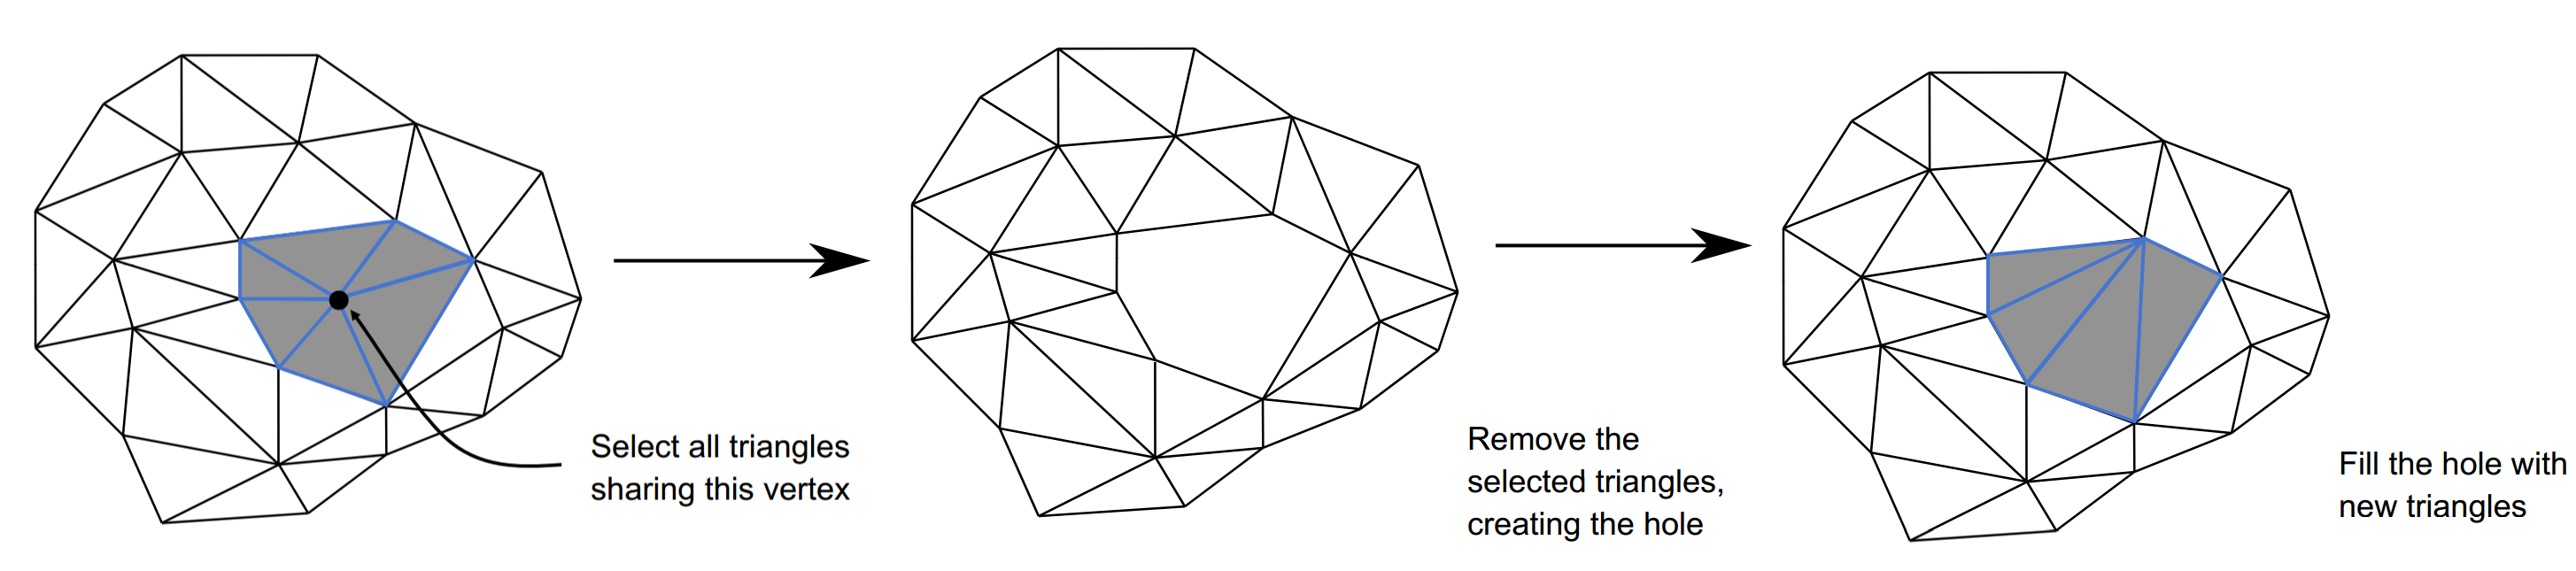
\includegraphics[width=.8\textwidth]{vertex_remove.png}
    \caption{通过顶点删除的操作简化网格,图来自\cite{mesh-simp}}
    \label{fig:rm-vertex}
\end{figure}
\begin{figure}[htbp]
    \centering
    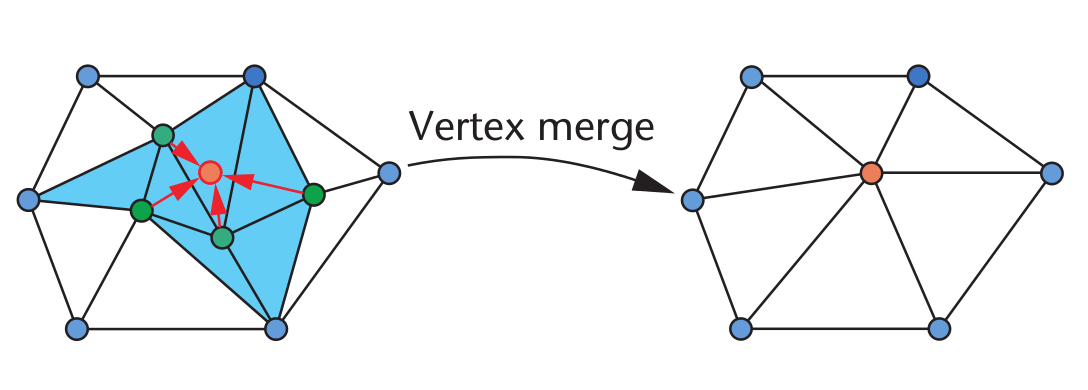
\includegraphics[width=.8\textwidth]{vertex_clustering.png}
    \caption{通过顶点聚簇合并的操作简化网格,图来自\cite{mesh-simp}}
    \label{fig:clu-vertex}
\end{figure}
%% 对于国内硕士学位论文来说,
%% 一般较少研究完全无前人探索的领域,
%% 所以有必要交待前人在此做出的努力和尝试。
%% 同样,请提供数据和引用保证严谨。

%% 为避免引起评阅老师判定有凑篇幅之嫌,
%% 请有针对的描述前人研究的不足之处,
%% 做到``有破有立''。
%% \def\theequation{S\arabic{equation}}
在网格简化算法中,我们通常用Hausdorff距离被用来作为衡量简化结果与原网格之间的误差(以下Hausdorff距离公式,引用自$https://en.wikipedia.org/wiki/Hausdorff\_distance$)。单个
点$x\in\mathbb{R}^3$到一个三角网格$F$的 Hausdorff 距离定义为:
\begin{equation}
  d(x, F) = \underset{y\in F}{inf}||x-y||
  \label{eq:v2f-haus}
\end{equation}
这里y是三角网格F表面上的任意一点,inf表示取最小值。定义三角网格$F_1 \to F_2$的最大Hausdorff距离为:
\begin{equation}
  \rho_{max}(F_1,F_2)=\underset{x\in F_1}{sup}(x,F_2)
  \label{eq:f2f-max-haus}
\end{equation}
这里sup表示取最大值。定义三角网格$F_1 \to F_2$的平均Hausdorff距离为:
\begin{equation}
  \rho_{mean}(F_1,F_2)=\underset{x\in F_1}{avg}(x,F_2)
  \label{eq:f2f-mean-haus}
\end{equation}
这里avg表示取平均值。定义三角网格$F_1 \to F_2$的Hausdorff距离的均方根(RMS)为:
\begin{equation}
  \rho_{rms}(F_1,F_2)=\underset{x\in F_1}{rms}(x,F_2)
  \label{eq:f2f-rms-haus}
\end{equation}
定义两个三角网格之间的双向最大Hausdorff距离和双向平均Hausdorff距离以及双向Hausdorff 距离的均方根分别为:
\begin{equation}
  \begin{array}{l}
    d_{H\_max}(F_1,F_2)=sup(\rho_{max}(F_1,F_2), \rho_{max}(F_2,F_1))\\
    d_{H\_mean}(F_1,F_2)=sup(\rho_{mean}(F_1,F_2), \rho_{mean}(F_2,F_1))\\
    d_{H\_rms}(F_1,F_2)=sup(\rho_{rms}(F_1,F_2), \rho_{rms}(F_2,F_1))
  \end{array}
  \label{eq:ff-haus}
\end{equation}
相同的Hausdorff距离下,比较网格的简化程度(顶点或三角面片数量),或者相同的简化程度下比较简化之后的网格和原网格之间的Hausdorff距离是比较两个网格简化算法的重要依据。根据给定不同的网格简化条件,当前的简化算法可以分为两类:$Min−\#$类算法和$Min−\varepsilon$类算法。$Min−\#$类算法给定一个误差范围ε以及其计算方式,在保证简化的结果与原模型间的误差不允许超过ε的条件下做网格简化。$Min−\varepsilon$类算法则在给定一个最终的简化结果的顶点或三角面片数量的条件下,尽可能地最小化简化结果与原网格之间的误差。\par
在所有$Min−\varepsilon$类简化算法中,Michael Garland等人提出的QEM算法\cite{qem1}凭借其高效简单效果好,成为较流行的网格简化算法之一。现在,我们可以下载到实现该算法的开源应用QSlim。在该算法中,每个三角网格模型被视为是由很多个有限的平面所构成。该算法的主要思想是在做顶点合并时,最优化(最小化)每个顶点到其所属平面集合的距离平方和,从而将降低每次简化带来的误差。与该算法相似的还有Peter Lindstrom等人提出的MemorylessSimplification,也是通过贪心的策略迭代地合并顶点。与前者不同的是该算法将上一次的结果作为参考,最优化(最小化)的是新网格与参考网格所构成的体积。该算法通过这种保体积的策略,得到了比QEM算法更优的简化效果。由于在确定一个定点对的合并点位置时,需要最优化体积,因此需要消耗的时间是QEM的10倍左右。\par
为了满足在高精度范围内简化网格的需求,产生了$Min−\#$类算法,其中最具代表性的算法之一是Jonathan Cohen等人提出的一种基于内外壳的网格简化算法\cite{simp-envlop}。在用户给定最大误差$\varepsilon$的条件下,该算法首先生成与原始网格距离为$\varepsilon$的内外壳边界,然后在保证新生成的三角面片不与内外壳相交的条件下做顶点合并。而在同样给定最大误差$\varepsilon$的条件下,Borouchaki等人提出了一种能够直接约束Hausdorff距离不超过$\varepsilon$的网格简化算法——MMGS,而且在MMGS中通过翻面和定点光顺优化了定点的位置,使得结果更加光顺。在2015的SIG上Manish Mandad等人发表了一种将网格重建和基于内外壳简化算法相结合的网格近似算法,该算法也是本文主要参考的算法。该算法能在给定内外边界采样点的情况下,先通过世面体化重建出一个夹在内外壳之间的原网格近似,在此基础上通过消边来简化这个四面体结构,从而生成一个尽可能简化的网格去近似原网格,我们将在后续的章节中详细介绍。
\section{本文工作}
通常我们以以下几个方面来评价一个网格简化算法:
\begin{enumerate}[(1)]
\item 相同误差下简化程度的高低和相同顶点数量下简化误差的大小;
\item 能否较好地保持原网格的法向信息;
\item 算法是否高效简单。
\end{enumerate}
现在的一些主流的方法,虽然能够较好地满足一般用户的需求。但是均无法做到能够鲁棒地处理各种输入数据的同时能够严格地控制简化误差。而最近 Manish Mandad等人提出的网格同坯近似算法,很好地做到了前三点。我们在实现其算法的基础上,对其可能存在的不足做了分析,并实现了我们的改进。Manish Mandad等人提出的网格同坯近似算法大致可以分为以下几个步:细化、简化误差边界、镶嵌0等值点、简化0等值面和消除所有可能消除的边。该算法以在误差空间Ω的内外边界(内外壳)上密集的采样点S来作为输入数据,在细化阶段,以这些采样点的包围球的3D Delaunay三角化作为初始化,在这个三角化的每个四面体上维护一个线性差值函数,其中包围球和外壳采样点的值定为1,内壳采样点的值定为-1。然后不断地往这个三角化中加入内外边界的采样点,直到这个差值的0等值面(所有差值为0的点构成的面)能够将所有的内外采样点区分开,这样就得到了一个原误差空间的近似Γ。简化误差边界,就是在保持0等值面仍能够区分内外采样点的条件下去尝试消除误差空间Γ边界上的边。在镶嵌0等点,则是将所有在边上的0等值点插入到这个三角化中。在镶嵌0等值点之后,就得到了显示的0等值面——原网格的一个近似,不过这0等值面还不够简单,我们需要尝试消除每一条由0等值点所构成的边,在保持0等值面任然能够将内外采样点区分开的条件下。之后为了进一步简化,可以在该条件下,继续消除所有可能消除的边。由于该算法始终确保0等值面能将内外采样点分开这个条件,因此能够严格地控制误差。并且在整个简化过程中依次遍历所有可能消除的边,在消边时则通过对附近空间采样去寻找可能的合并点的位置,因此,在简化结果上,与以往的算法比较具有明显优势。然而,在初始化重构网格时用的3D Delaunay三角化,虽然这样能够拥有较好地质量,但并没有考虑到原三角网格本身存在的各项异性,从而使得接下来需要经过消边来获得这个特性。为了获得一个更好的初始化,我们需要一个各项异性的3D Delaunay三角化。我们根据原三角网格的曲率信息,对其做一个形变,在形变空间中做3D Delaunay三角化,对应到原空间中我们就得到了一个各项异性的三角化。这样的初始化,不仅大大简化了细化的结果——得到了一个更好的初始化状态,而且使得最终我们能够在给定的误差范围内得到一个顶点数量更少的结果。
%% 此部分必须详细描述,
%% 必要时可划设小节。
%% 国外学位论文的Introduction章基本仅阐述此内容。
%% 为研究开展的相关工作和实验,
%% 此间遇到何难处及对应的解法。
%% 对论文研究领域不甚了解的评阅老师,
%% 希望从摘要和此小节尽可能的了解最多信息。


\section{论文的内容和结构安排}
首先我们介绍了现阶段三角网格简化在计算机图形学和计算机辅助设计中的重要意义,以及现阶段三角网格模型简化的背景,并介绍了现在国内外的一些研究成果和算法以及它们各自的优势和不足。然后提出了我们认为的三角网格简化的几个目标,并介绍了我们改进的基于内外壳的网格简化算法及其具体实现。最后是我们对三角网格简化工作的总结和展望。\par
本文的章节安排如下,第一章介绍网格简化的背景和国内外对网格简化的研究现状,以及本文的主要工作;第二章对我们所参考的一些主流的网格简化算法做了一个详细地介绍和分析;第三章,详细描述了 Manish Mandad 等人提出的基于内外壳的网格近似算法;第四章,我们基于 Manish Mand 提出的算法的改进;第五章,我们的算法的结果展示;第六章是总结和展望。
 % 绪论
%%!TEX root = ../main.tex

\chapter{相关网格简化算法及其分析}
\section{QEM 网格简化算法}
QEM算法凭着其简单高效的特点是网格简化算法中主流算法之一。在QEM算法中,每一个模型被视为是由很多个离散的有限平面所组成,而模型上的每一个顶点就是其一环邻域(周围的一圈)平面的交点。因此,我们将顶点$v=[x,y,z,1]^T$和一系列平面关联起来,相当于每一个顶点$v$都应该在一个平面集合$planes(v)$的每个平面上。每一个$plane(v)$都可以表示为$pTv=0,p=[a,b,c,d]T,a2+b2+c2=0即ax+by+cz+d=0$$,从而该顶点到这个平面plane(v)的距离的平方可表示为(pTv)2即vTppTv,每一个顶点到其平面集合的距离平方和为

%\include{contents/whyla}
%!TEX root = ../main.tex

\chapter{网格同坯近似算法}
在上一章中我们介绍了现有的四种比较主流的网格简化算法。就简化结果而言,相对复杂的基于内外壳的简化算法不仅能够更好地控制简化误差,而且能够在相同误差下获得更高的简化程度,在相同的简化程度下获得更低的误差。最近Manish Mandad等人将网格重建和带有内外壳的网格简化算法进行了有机地结合,提出了一种新型的鲁棒的网格同坯近似算法\cite{isotopic-appro}。与其他基于内外壳的网格简化算法不同,该算法以给定误差空间的内外边界上的采样点为输入,先重建再简化,因此,对原网格的要求更低——只要能通过原网格生成比较好的内外边界采样点如图\ref{fig:iso-appro-robust}。该算法通过空间四面体化,并通过这个四面体网格中线性差值维护一个空间中的误差函数$\epsilon(s)$,来控制简化结果与原模型之间的误差在用户给定的范围内。该算法大致可以分为以下步骤:
\begin{enumerate}[(1)]
  \item 细化,构建误差空间Ω的近似Γ;
  \item 简化误差空间Γ的边界;
  \item 镶嵌 0-等值点;
  \item 简化 0-等值面;
  \item 所有可能的简化。
\end{enumerate}
\begin{figure}[htbp]
    \centering
    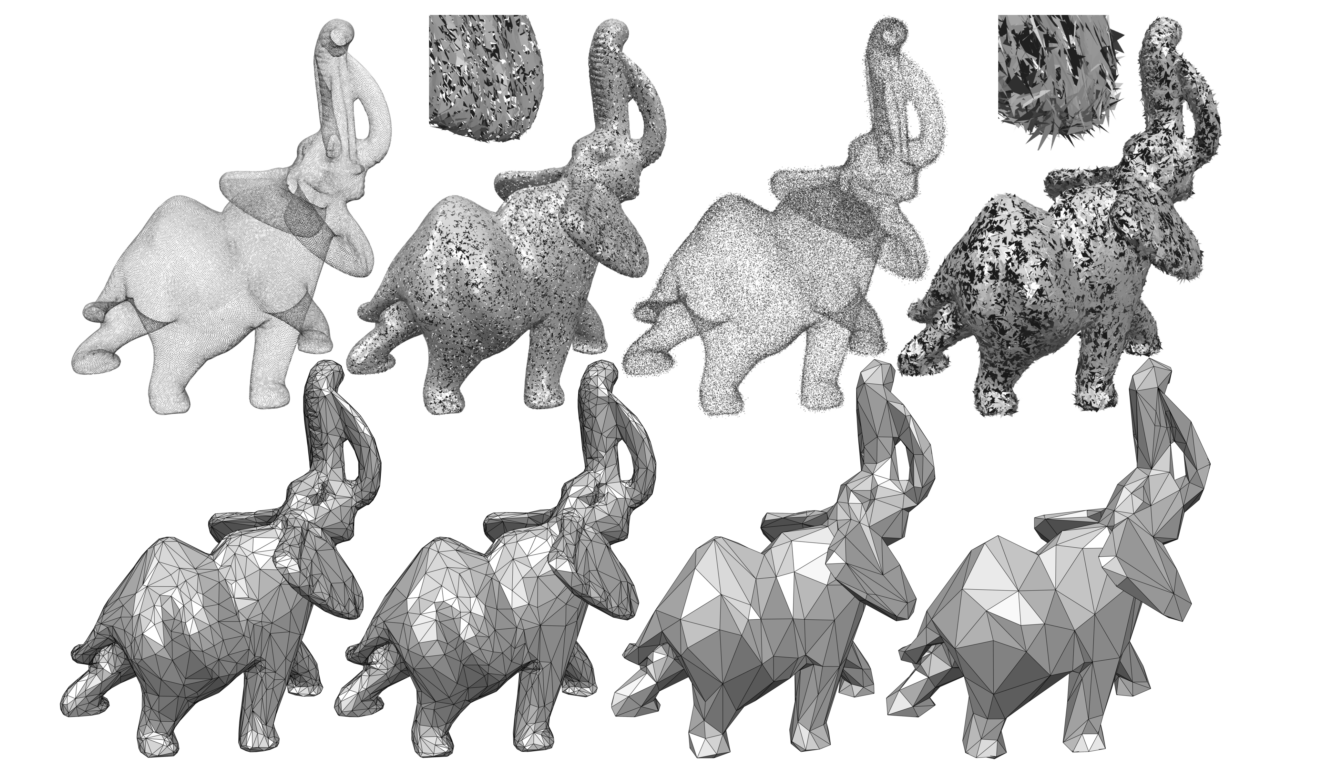
\includegraphics[width=.8\textwidth]{iso_appro_robust.png}
    \caption{网格同坯近似算法能鲁棒地处理带有噪声的输入数据。从左到右分别是顶点集合,带有低噪声的三角面片集合,带有高噪声的顶点集合以及带有高噪声的三角面片集合。第二行是对这些数据的简化结果,图引用自\cite{isotopic-appro}}
    \label{fig:iso-appro-robust}
\end{figure}

\section{细化,构建误差空间Ω的近似Γ}
对于给定的误差空间为$\Omega$,算法以对误差空间$\Omega$的边界$\partial \Omega$上的一个密度为$\sigma$的采样(以每个采样点为圆心,以$\sigma$为半径的圆球,能够覆盖整个$\partial \Omega$)所得到的采样点集合S作为输入。算法假定这个误差空间只有两个边界,内边界和外边界,定义$S_0$为内边界采样点,$S_1$为外边界采样点,$S_{bs}$为包围球上的采样点。在S上定义一个参照函数:
\begin{equation}
  \begin{split}
    F(s) &= -1, s\in S_0\\
    F(s) &= +1, s\in S_1\\
    F(s) &= +1, s\in S_{bs}
  \end{split}
\end{equation}
然后以$\Omega$的包围球上的采样点$S_{bs}$作为初始化顶点,做一个四面体化,得到四面体网格$\tau$。在$\tau$上针对每一个四面体维护一个线性差值函数:
\begin{equation}
  f(s) = \sum_{i=0}^3 w_iF(s_i), s\in tet(s_0, s_1, s_2, s_3), s_i \in \tau
\end{equation}
这里,$tet(s_0, s_1, s_2, s_3)$是由这四个顶点所构成的四面体,$w_i$是顶点s在这个四面体上的重心坐标分量。所谓重心坐标是指对于四面体$tet(s_0, s_1, s_2, s_3)$中的一个顶点s,我们可以通过这四个点的加权来得到s的坐标值即:
\begin{equation}
  \begin{split}
  \sum_{i=0}^3 w_i s_i &= s\\
  \sum_{i=0}^3 w_i &= 1
  \end{split}
  \label{eq:err-constraint}
\end{equation}
这样,我们就可以得到每一个内外壳上的采样点的对应函数值,定义所有$f(s)=0$的点的集合为$\mathcal{Z}$即0-等值面,而当内外采样点的$f(s)$函数值与参照函数$F(s)$的函数值相差不超过1的时候,这个0-等值面$\mathcal{Z}$能够正确地将$S_0$和$S_1$的采样点区分开,也即0-等值面不会超越误差空间(如图\ref{fig:isotopic-appro})。因此,在采样点S上定义一个误差函数:
\begin{equation}
  \epsilon(s) = \lVert f(s)-F(s) \rVert
\end{equation}
从而误差约束条件转化为:
\begin{equation}
  \forall s \in S, \epsilon(s)<1
\end{equation}

\begin{figure}[htbp]
    \centering
    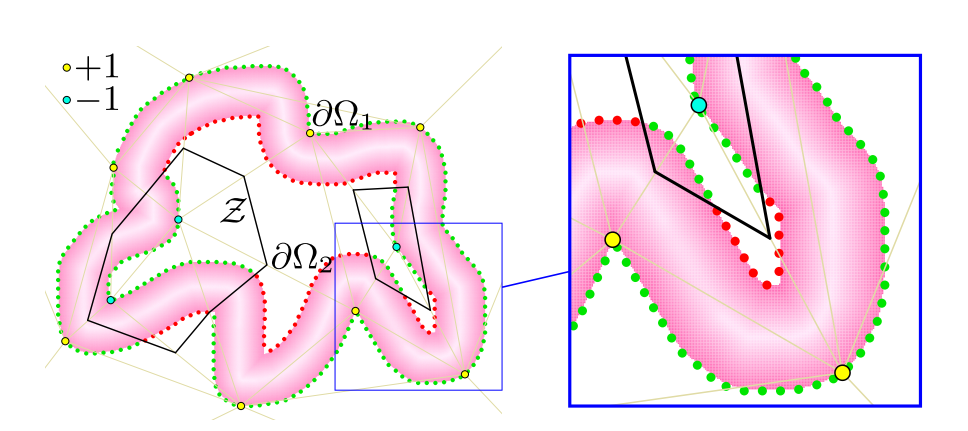
\includegraphics[width=.7\textwidth]{classification.png}
    \caption{图中绿色的点已经被0-等值面正确地分开,而红色的点未被正确地分开,图来自\cite{isotopic-appro}}
    \label{fig:isotopic-classification}
\end{figure}

\begin{figure}[htbp]
    \centering
    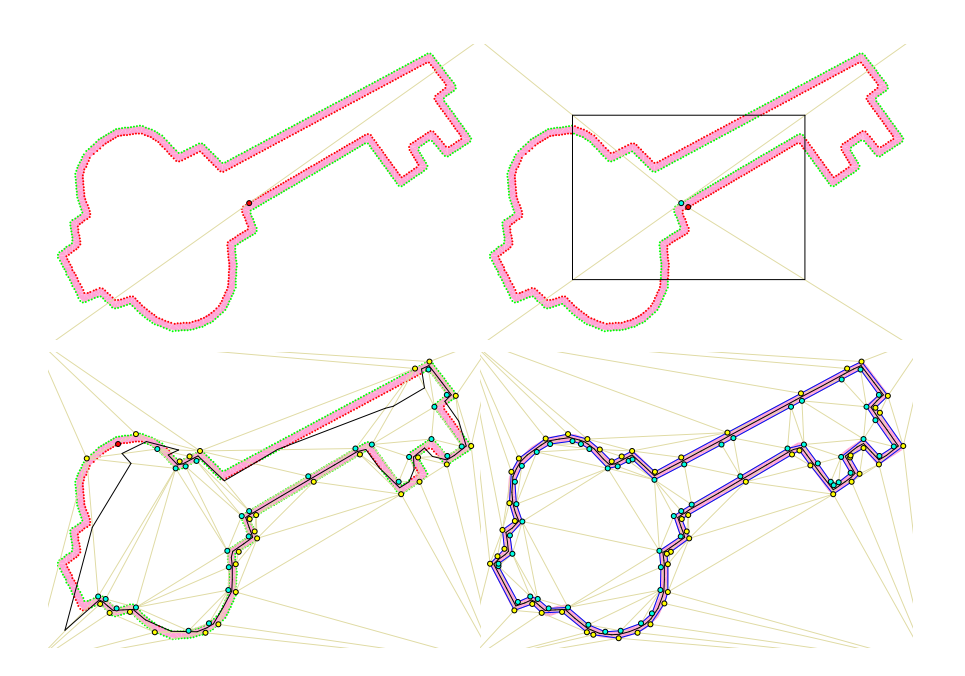
\includegraphics[width=.7\textwidth]{refine.png}
    \caption{细化的过程——逐渐地加入采样点直到所有的采样点能够被0-等值面正确地区分开,图来自\cite{isotopic-appro}}
    \label{fig:refine}
\end{figure}

\par 在细化阶段基本思路是:使用贪心的策略不断地选取$s \in S,\epsilon(s)$最大的顶点加入到$\tau$中,并重做四面体化直到直到$\tau$达到这个约束条件(如图\ref{fig:refine})。不过为了保持法向的质量,尽可能避免简化后的网格可能会出现法向翻转的问题(如图\ref{fig:normal-cond}),需要添加一个额外的法向约束条件:在每一个四面体上定义的线型差值函数不仅能够正确地区分在该四面体内的S中的采样点,而且当该四面体缩小到一个比例$\alpha$后,该线性差值函数也能够区分内外壳上离缩小的四面体的四个顶点最近的采样点。在整个细化的过程中,依次判断误差约束条件,以及法向约束条件是否得到满足。
\begin{figure}[htbp]
    \centering
    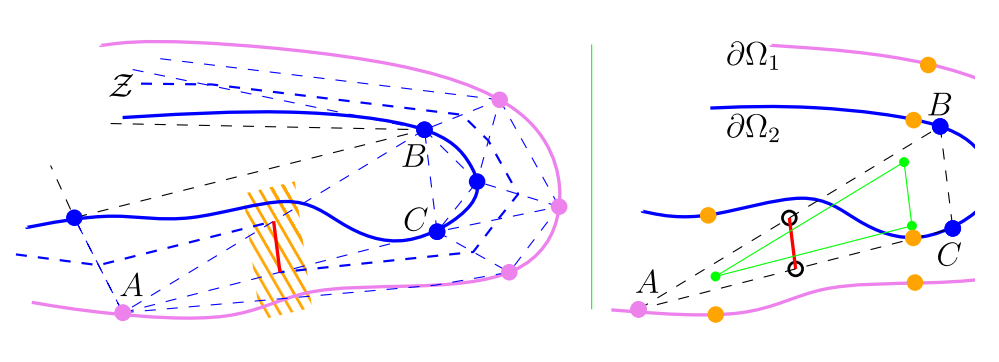
\includegraphics[width=.7\textwidth]{normal_cond.png}
    \caption{由于三角化不合理导致的法向不合理的情况(左图红色边)。右图是对法向是否合理的一个检测,红色的边并不能将绿色三角形($\triangle ABC$缩小一定比例之后的三角形)的三个顶点最近的内外壳采样点(橘黄色的顶点)正确地划分开,图来自\cite{isotopic-appro}}
    \label{fig:normal-cond}
\end{figure}
为了得到一个质量相对较好的四面体网格$\tau$(尽量避免细长的四面体出现),使用3D Delaunnay三角化来为空间中的顶点构建四面体网格。对于$\mathbb{R}^3$上的顶点集合S,其3D Delaunay三角化$(DT)$的结果$D(S)$是一个满足对于任意一个$D(S)$上的四面体,没有其他顶点落在它的外接球内部(如图\ref{fig:2d-delaunay})。对于$S$上的一个3D三角化$\tau$,对于一个三角面片$f \in \tau$,若$f$与由其所构成的四面体的任一外接球中的顶点均没有边相连,那么我们所这个三角面片f是局部Delaunay的。如果$\tau$中的所有三角面片都是局部Delaunay的,那么$\tau \equiv D(S)$。3D Delaunnay三角化的一个重要特点是能够最小化四面体网格中四面体的最大外接球。因此,3D Delaunay三角化能够尽可能避免一些狭长的四面体的出现,获得质量较好地四面体网格。在细化结束后,就得到了一个原误差空间$\Omega$的近似$\Gamma$。也得益于3D Delaunay三角化,对于不满足法向约束条件的四面体,可以选取离该四面体外接球球心最近的采样点加入到四面体网格$\tau$中,然后更新四面体网格$\tau$。由于采用3D Delaunay三角化的性质,加入这样的点会破坏原不满足法向约束条件的四面体(在新的题网格$\tau$中,这四个点不构成一个四面体),从而达到了消除不满足法向约束条件的四面体的功能。
\begin{figure}[htbp]
    \centering
    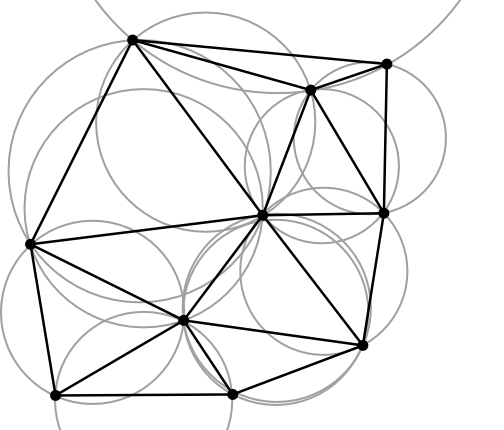
\includegraphics[width=.5\textwidth]{2d_delaunay.png}
    \caption{2D 上的 Delaunnay 三角化示意图,引用自\cite{wiki}}
    \label{fig:2d-delaunay}
\end{figure}

\section{误差边界$\partial \Gamma$的简化}
在初始化得到了一个满足误差控制要求的四面体网格$\tau$,通过消除这个近似误差空间$\Gamma$的边界$\partial \Gamma$上的边来简化$\partial \Gamma$。首先需要保证简化过后的四面体网格$\tau$仍然是一个有效的四面体网格:
\begin{enumerate}[(1)]
  \item 四面体网格的拓扑结构是有效的(保证不会出现不属于任何四面体的面等);
  \item 四面体网格是包围球空间的一个有效的填充,即不存在相互交叉的四面体。
\end{enumerate}
为了保证简化后的τ足第一个条件,需要保证我们消除的边需满足Dey等人提出的Link Condition\cite{link-cond},而对于第二个条件需要使得消除的边的合并点落在这条边的Kernel Region中。除了上述两个基本的条件外,还需要保简化满足误差约束条件\eqref{eq:err-constraint},以及为了维持法向质量所加的法向约束。

\subsection{Link Condition}
借鉴Dey等人对保持拓扑有效性的消边的研究,在$\tau$上做消边操作时,需要判断该边是否满足Link Condition。一个由k+1个独立的点构成的凸包$\sigma$,被称为k-simplex,比如 0-simplex ——点,1-simplex ——线段。$\sigma$上的一个非空子集t,称为$\sigma$的face,而相对的$\sigma$是t的coface。定义由有限个k-simplex构成的一个集合$\mathcal{K}$,称为simplical complex。这里的四面体网格$\tau$就是这样的一个simplical complex。假设B是一个simplical complex $\mathcal{K}$上的一个子集,则定义B的closure ——$\overline{B}$(如图\ref{fig:closure}),为包含B中所有face的最小simplical complex。而B的star ——$St B$(如图\ref{fig:star}),定义为包含B中每一个simplex的star的并集,一个simpex的star即为该simplex的coface。而Lk(B):$Lk B = \overline{St B} - St \overline{B}$(如图\ref{fig:link})。\par

\begin{figure}[htbp]
    \centering
    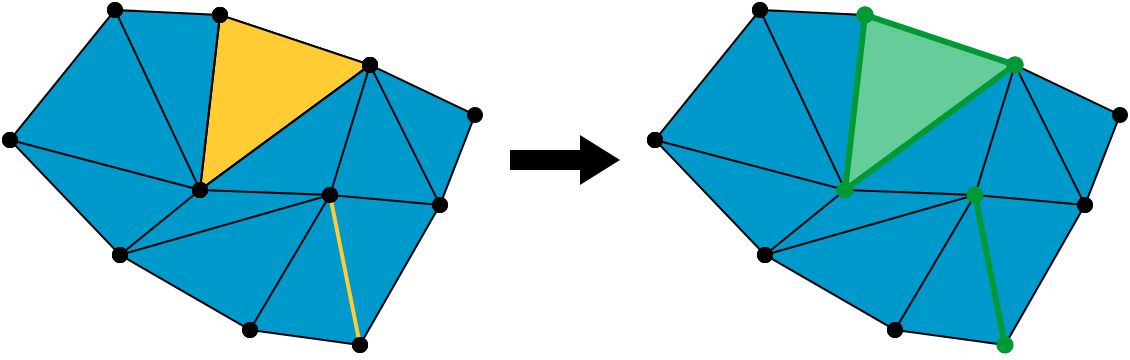
\includegraphics[width=.7\textwidth]{simplicial_complex_closure.png}
    \caption{2D三角网格上的closure示意图,图引用自\cite{wiki}}
    \label{fig:closure}
\end{figure}
\begin{figure}[htbp]
    \centering
    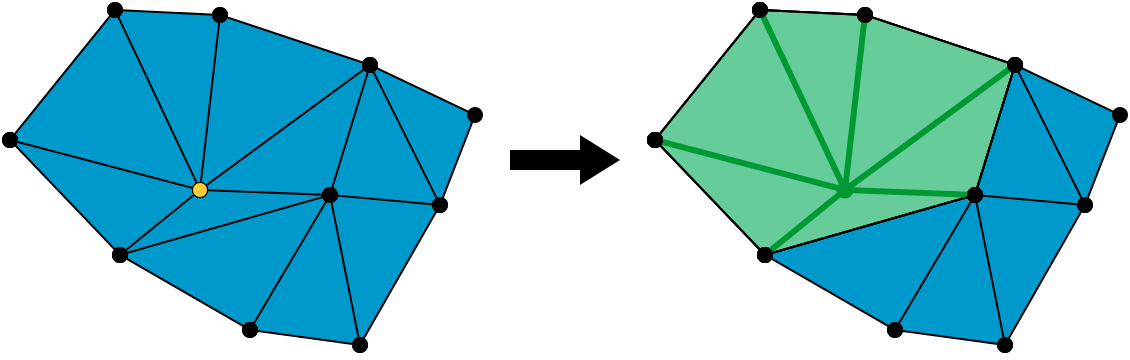
\includegraphics[width=.7\textwidth]{simplicial_complex_star.png}
    \caption{2D三角网格上的star示意图,图引用自\cite{wiki}}
    \label{fig:star}
\end{figure}
\begin{figure}[htbp]
    \centering
    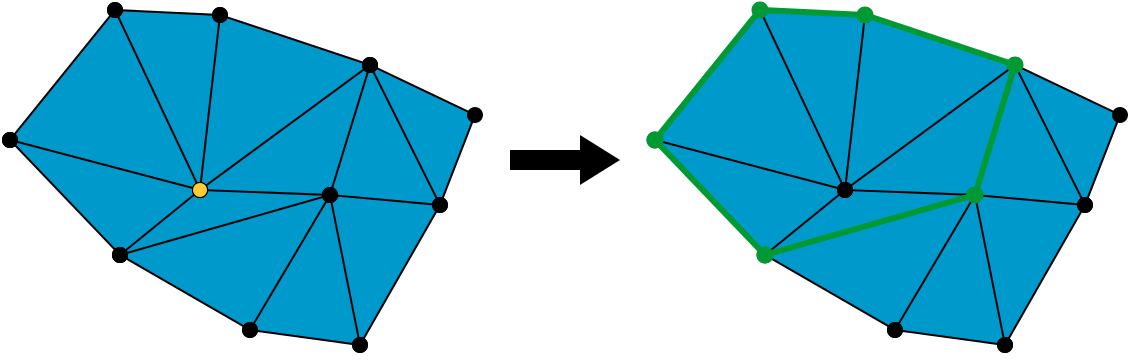
\includegraphics[width=.7\textwidth]{simplicial_complex_link.png}
    \caption{2D三角网格上的link示意图,图引用自\cite{wiki}}
    \label{fig:link}
\end{figure}
从而边AB上的Link Condition定义为$Lk(A) \cap Lk(B) = LK(AB)$。从Link Condition中我们可以直观地发现,对于2D空间中的一个点A其Lk(A)为顶点A的一环邻域的边界上的顶点和边,而$Lk(AB)$则是包含边AB的三角形的另一个顶点,边AB的Link Condition是否满足等价于A和B各自一环邻域的边界不能相交于一条边,否则AB合并之后该边将成为一条孤立的边(不属于任何三角形,如图\ref{fig:2d-link-cond})。类似的对于3D空间上AB的Link Condition是否满足等价于A和B各自的一环邻域的边界不能相交于一个面,否则AB合并之后该面将成为一个孤立的面(不属于任何四面体,如图\ref{fig:3d-link-cond})。
\begin{figure}[htbp]
    \centering
    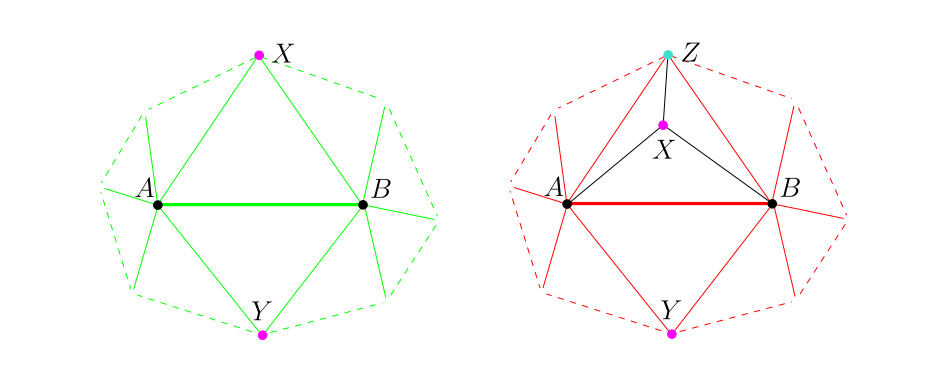
\includegraphics[width=.7\textwidth]{2d_link_cond.png}
    \caption{2D三角网格上的Link Condition示意图,对于边AB,左图满足Link Condition,右图不满足Link Condition,图引用自\cite{isotopic-appro}}
    \label{fig:2d-link-cond}
\end{figure}
\begin{figure}[htbp]
    \centering
    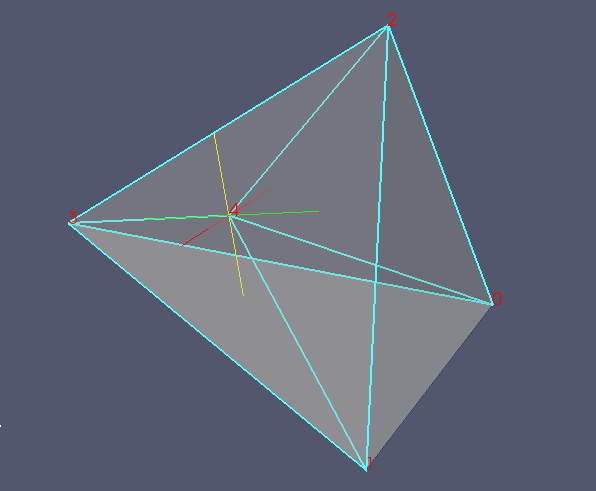
\includegraphics[width=.5\textwidth]{3d_link_cond.png}
    \caption{3D三角网格上的Link Condition示意图,顶点1和3不能被合并,若顶点1和3合并,则会出现一个不属于任何四面体的三角面片024}
    \label{fig:3d-link-cond}
\end{figure}

\subsection{Kernel Region}
为了保证消边之后$\tau$仍然是包围球空间的一个有效填充,即不会产生四面体相互交叉的情况,需要保证得新生成的四面体是边PQ——环邻域的空间(由包含P或Q的四面体构成的空间)的有效填充。因此,PQ的合并点必须落在PQ的邻域空间的边界的每一个三角形内侧。我们定义该空间为边PQ的Kernel Region——$K_\tau(PQ)$(如图?是2D的Kernel Region示意图)。
\begin{figure}[htbp]
    \centering
    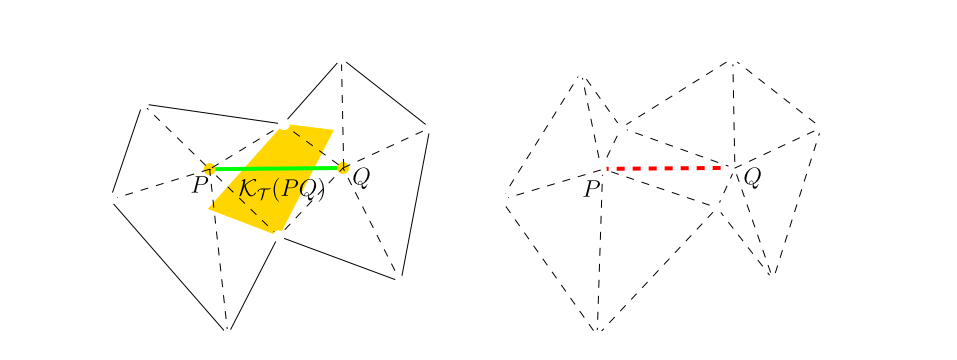
\includegraphics[width=.8\textwidth]{kernel_region.png}
    \caption{在二维中一条边的PQ的Kernel Region为PQ的一环邻域的三角面片边界上,每一条边所对应的直线的内侧(PQ这一侧)的交集,图引用自\cite{isotopic-appro}}
    \label{fig:kernel-region}
\end{figure}
\par 在对$\partial \Gamma$进行消边时,从内外壳的采样点中选取合并点。除了需要满足保持四面体网格$\tau$的有效性外,还需要保证满足误差控制条件$\forall s \in S, \delta(s) < 1$。因此,需要对$K_\tau (PQ) \cap S$中所有的点,逐个判断若合并到该点后,新生成的四面体空间中所有的采样点是否满足$\delta(s) < 1$,若满足则合并到这个点,否则继续尝试下一个点。若$K_\tau (PQ) \cup S$所有的点都无法保持$\delta(s) < 1$这个条件,则放弃消除这条边。和其他简化算法类似,为了找到一个更优的合并点的位置,使得误差更小,可以对所有的采样点根据其到PQ的2环邻域的每一个0-等值三角形所在平面的距离平方和由小到大做一个优先级排序。
\subsection{0-等值面的生成}
当误差边界$\partial \Gamma$简化完成之后,将$\tau$中每一条由连接内外边界$(\partial \Gamma_0, \partial \Gamma_1)$的边的中点——0-等值点嵌入到这个四面体中并细分这个四面体网格,从而得到由0-等值点构成的0-等值面$\mathcal{Ζ}$,现在$\mathcal{Z}$是在误差空间$\Omega$中原网格的一个同坯近似(如图\ref{fig:mutual-tessellation})。
\begin{figure}[htbp]
    \centering
    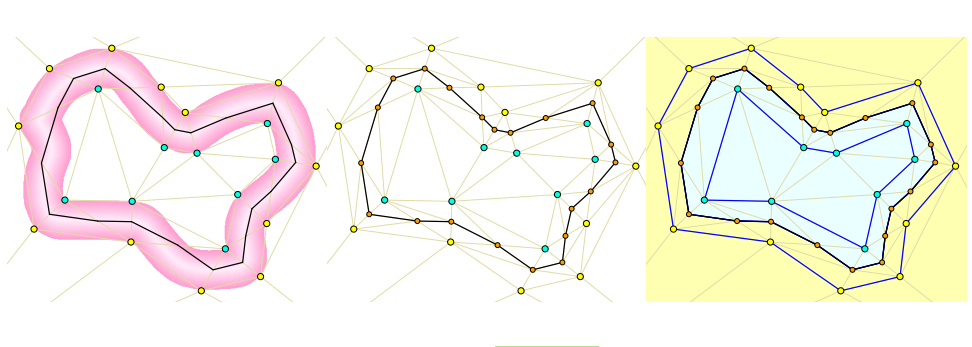
\includegraphics[width=.8\textwidth]{mutual_tessellation.png}
    \caption{在二维上的0等值点嵌入:左图为在0-等值点嵌入之前;中间图为0-等值点嵌入之后;右图显示了$\partial \Gamma$的边界线蓝色线,以及0-等值线黑色线,以及函数$f(s)$的取值情况,黄色区域$f(s) > 0$,淡蓝色区域$f(s) < 1$,图引用自\cite{isotopic-appro}}
    \label{fig:mutual-tessellation}
\end{figure}

\subsection{所有可能的简化}
由于$\Gamma$是原误差空间$\Omega$的一个简化近似,因此,0-等值面的简化可能无法充分利用$\Omega$的空间(如图\ref{fig:tol-small})。为了尽可能充分地利用误差空间,可以通过尝试消除由0-等值点或边界上的点构成的边来调整0-等值点的位置,并扩大0-等值面上的边的Kernel Region,从而达到进一步简化的目的(如图\ref{fig:all-edges-collapse})。当所有简化都结束之后,最终的0-等值面就是我们的简化结果。

\begin{figure}[htbp]
    \centering
    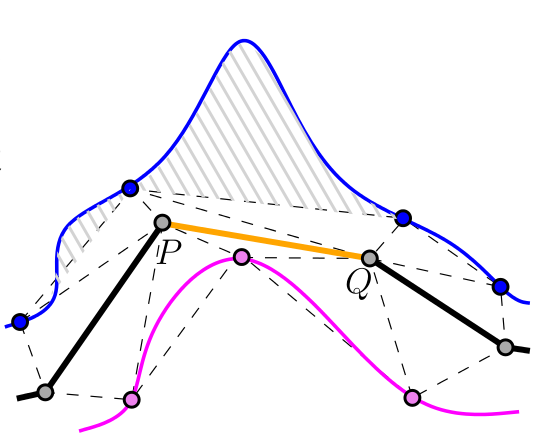
\includegraphics[width=.5\textwidth]{tol_small.png}
    \caption{图中阴影部分空间无被充分利用起来,图引用自\cite{isotopic-appro}}
    \label{fig:tol-small}
\end{figure}

\begin{figure}[htbp]
    \centering
    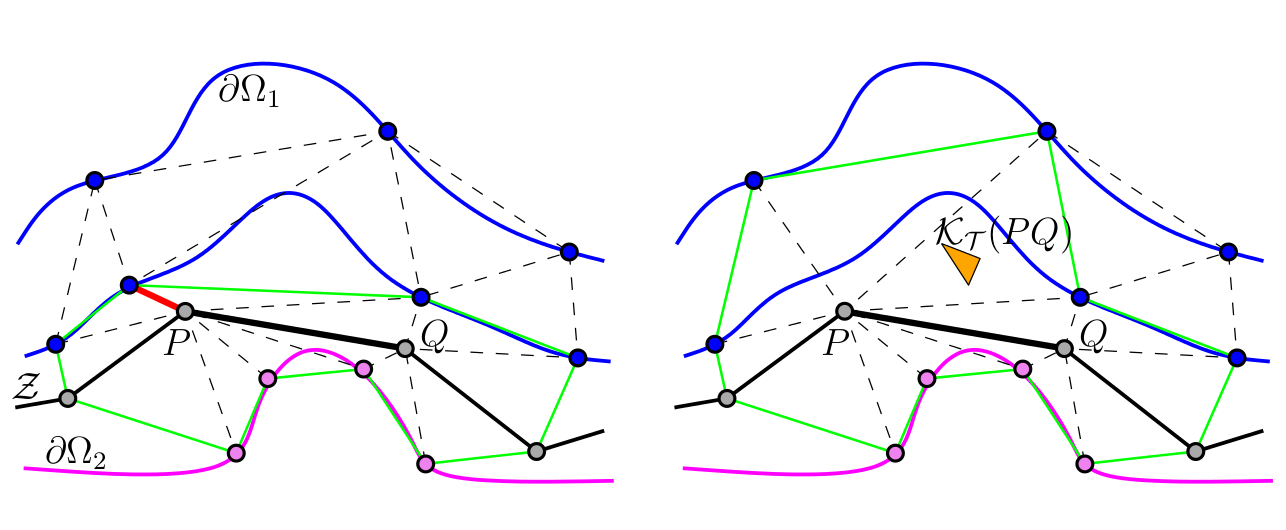
\includegraphics[width=.9\textwidth]{zb_collapse.png}
    \caption{通过消除所有可能的边来进一步简化网格。左图中边PQ由于Kernel Region为空而无法消除,在右图中通过消除左图中的红色边,PQ的Kernel Region变为橙色的区域(不为空),从而增大了PQ消除的可能性。图引用自\cite{isotopic-appro}}
    \label{fig:all-edges-collapse}
\end{figure}

\section{本章小结}
本章详细介绍了Manish Mandad等人提出的网格同坯近似算法\cite{isotopic-appro}。本章首先简述了该算法的其特点,并详细介绍了其主要步骤。该算法以误差空间$\Omega$的边界上的采样点S作为输入。以S的包围球上的顶点初始化顶点,利用 3D Delaunay三角化建立起一个四面体网格$\tau$,并在这个四面体网格上维护一个误差函数$\epsilon(s)$,贪心地从S中选取误差最大的顶点插入到$\tau$中,直到S中所有点的误差不超过1。然后在保持$\tau$有效、保持误差约束和保持法向约束条件的前提下、通过简化误差边界,得到一个更加稀疏的误差空间$\Omega$的近似。再通过嵌入0-等值点得到显示的0-等值面。最后通过简化0-等值面和所有可能的简化得到最终的简化结果。
%% 通过阅读上一章节,
%% 相信您已基本配置好了自己的编辑环境,
%% 了解了如何正确编写各级章节、段落和子段落,
%% 容易引起编译出错的逃逸字符。

%% 从上一章出现过的有序列表、外部图片和代码环境中,
%% 您应该已经发现,
%% 使用命令\texttt{$\backslash$begin\{xxxx\}}可以开始一段新的布局环境。
%% 这一章将系统地阐述计算机类的学位论文需要排版的元素的编写方法。
%% 主要包括以下排版要素:
%% \begin{itemize}
%%     \item 列表环境(包括有序、无序、定义三种列表)
%%     \item 插图和表格
%%     \item 代码环境
%%     \item 数学和算法环境
%% \end{itemize}

%% 这一章只涉及为完成此排版环境的宏包的最基本使用方法,
%% 本章尽量覆盖论文写作中的大部分场景,
%% 如有特殊需求,请仔细阅读相关宏包手册并求助于国内外TeX社区及问答网站。

%% \section{列表环境}

%% 列表环境有三种,
%% 类似与HTML的\texttt{<ol>},
%% \texttt{<ul>},\texttt{<dl>}
%% 三个标签。
%% 以下是一个定义列表环境:
%% \begin{description}
%%     \item[有序列表] enumerate 默认从阿拉伯数字1开始编号,如需更改请搜“重定义列表”
%%     \item[无序列表] itemize 默认圆点标记,尽量少用此类列表
%%     \item[定义列表] description 语义上用于作一系列简短的解释
%% \end{description}

%% 列表可以嵌套,比如:
%% \begin{enumerate}
%% 	\item 第一级列表
%% 	\item 第一级列表
%% 	\begin{enumerate}
%% 		\item 第二级列表
%% 		\item 第二级列表
%%         \begin{itemize}
%%             \item 第三级列表
%%             \item 第三级列表
%% 		\end{itemize}
%% 		\item 第二级列表
%% 		\item 第二级列表
%% 	\end{enumerate}
%% \end{enumerate}

%% \section{插图环境和浮动体}

%% 相信您在上一章的探索学习中已经基本掌握了如何插入图片的方法,
%% 但可能仍存疑虑。
%% 所以现在先简单介绍浮动体的概念以助您理解插图环境的布局规则,
%% 最后再介绍子图的排布以应对您更高的布局需求。
%% % 关于绘图,本文将在后续章节讲述
%% % 活用引用,让评阅老师随处移动
%% 关于图的绘制,本文将在\ref{how-to-plot} 继续讲述。

%% 当一个图片或表格太大在当前页面无法继续排布时,
%% 一种解决方案就是新开一页再排布(Word 默认使用此种)。
%% 这个方法在页面上留下分空白,十分不美观。
%% \LaTeX 的默认解决方案是把它们“浮动”到下一页,
%% 与此同时使用后续正文文本填充当前的空白。

%% 插图和表格在\LaTeX 排版中被默认当成浮动体对待,
%% 当排版引擎试图放置一个浮动体时,它将遵循以下规则:
%% \begin{enumerate}
%%     \item 浮动体的布局大小不得超过版心的大小,否则抛出Overfull Page错误
%%     \item 浮动体只会向后浮动,不会向前浮动
%%     \item 浮动体默认按照 h $\to$ t $\to$ b $\to$ p 的规则布局
%%     \begin{description}
%%         \item[h] 当前位置,如果本页所剩空间不够,这一参数无效
%%         \item[t] 浮动到下一页顶部
%%         \item[b] 浮动到下一页底部(脚注之下)
%%         \item[p] 浮动到一个允许出现浮动体的页面上
%%         \item[!] 忽略浮动体放置的大多数内部参数\footnote{作者也不太懂}
%%     \end{description}
%%     \item 设置 htbp 参数的顺序不会影响默认的规则顺序
%% \end{enumerate}

%% 在实践中,一般选用浮动规则[htbp], [tbp], [htp], [tp] 来完成浮动体布局。
%% 请不要使用单一参数布局,这样极有可能出现难解的浮动问题。
%% 不适当的浮动规则参数将导致浮动对象被放进一个队列中等待布局,
%% 这个队列的默认大小是18,如果队列超限,编译中会抛出一个Too Many Unprocessed Floats错误。
%% 如果一页图片太多,甚至几乎占满一个版心,
%% 您可以通过\texttt{$\backslash$clearpage}命令强制在此处必须排版完所有浮动体
%% 再排版之后内容,关于清除浮动等复杂主题,这里不再展开。
%% 此处只能建议插图尺寸不宜过大,插图密度不宜过大。
%% 考虑到图文混排的最佳视觉要求,
%% 可以待论文内容稳定下之后,仔细调整插图代码的位置,
%% 通过前置插图代码,强行“向后浮动”,保证插图和引用处足够近。

%% 关于模板对浮动体的设置,参看\texttt{zjuthesis.cls},
%% 搜索关键字“浮动体”找到对应配置。
%% 图片引用路径在\texttt{zjuthesis.cls}里定义的\texttt{graphicspath}里,
%% 默认情况下\\\texttt{$\backslash$includegraphics}命令从论文源码根目录搜索引用的图片,
%% 如果先在根目录里匹配到文件名,则不再前往定义路径搜索,
%% 当引擎无法找到您指定的图片资源时,会导致编译错误。
%% 注意引用的文件名包括文件后缀。

%% % 现在你可以随意更动此插图代码的位置来感受一下浮动体布局的规则
%% \begin{figure}[htbp]
%% 	\centering
%% 	\begin{subfigure}[b]{.45\textwidth}  % 注意此处的尺寸控制
%% 		\centering
%% 		\includegraphics[width = \textwidth]{xuejian.jpg}
%% 		\caption{仙三}\label{fig:subfig-samp1}
%% 	\end{subfigure}
%% 	\begin{subfigure}[b]{.45\textwidth}
%% 		\centering
%% 		\includegraphics[width = \textwidth]{wenhui.jpg}
%% 		\caption{仙三外}\label{fig:subfig-samp2}
%% 	\end{subfigure}
%% 	\begin{subfigure}[b]{.45\textwidth}
%% 		\centering
%% 		\includegraphics[width = \textwidth]{lingsha.jpg}
%% 		\caption{仙四}\label{fig:subfig-samp3}
%% 	\end{subfigure}
%% 	\caption{仙剑白学传}\label{fig:subfig-samp}
%% \end{figure}

%% 接下来描述一下子图的编写,
%% 在实际论文撰写过程中,
%% 经常遇到需要比较几组实验数据或场景的需求。
%% 此时,合乎语义的做法是为不同的组设置子图,
%% 而不是分别设图。

%% 多个子图组成一个单独的浮动体进行布局,
%% 共用一个总图题总引用,并可以有各自单独的子图题和交叉引用。
%% 本模板使用subcaption 宏包处理子图排版问题,如\autoref{fig:subfig-samp} 所示
%% \footnote{不要在正式论文排版过程中使用彩色区分类别,论文最终以灰度打印}。
%% 论文中不可像本文一般,
%% 平白无故地出现与行文毫无关联的图例,
%% 而且,必须有适当的文字内容对图例做出解释。
%% 比如比较分析从\autoref{fig:subfig-samp1} 到\autoref{fig:subfig-samp3}
%% 仙剑系列在白学梗方面的运用变迁。\footnote{往后数代仍有类似场景 -\_-\# (顔文字書込禁止!)}

%% 当准备插图资源时,应该尽可能保证插图清晰,背景透明。
%% 图中文字大小与文中接近,不小于脚注大小,不大于正文段落文字大小,
%% 框线宽度不大于2px。

%% 如果您曾关注过图片格式,
%% 应该知道图片在计算机中一般分为矢量图(\autoref{fig:vector})和位图(\autoref{fig:raster})两种类型。
%% 通俗地理解,矢量图通过几何属性存储信息,所以在缩放时保持图形的几何属性。
%% 而位图按像素点存储信息,在缩放时必然丢失信息。
%% 对于学位论文里的大部分为表达实验数据而描述的图例,最好使用矢量图绘制,
%% 以给评阅老师或后人精确地参考和还原实验。
%% 常用的矢量图格式有eps, pdf, svg 和 Adobe 系列的文件格式。
%% 其中\LaTeX 格式可以直接引用eps 和 pdf 格式的图片。

%% \begin{figure}[htbp]
%% 	\centering
%% 	\begin{subfigure}[b]{.45\textwidth}
%% 		\centering
%% 		\includegraphics[width = \textwidth]{vector.pdf}
%% 		\caption{矢量图}\label{fig:vector}
%% 	\end{subfigure}
%% 	\begin{subfigure}[b]{.45\textwidth}
%% 		\centering
%% 		\includegraphics[width = \textwidth]{raster.png}
%% 		\caption{位图}\label{fig:raster}
%% 	\end{subfigure}
%% 	\caption{Google Logo 的矢量图和位图比较}\label{fig:vector-raster}
%% \end{figure}


%% \section{表格}
%% 表格与插图一样,也是浮动体。
%% 在\LaTeX 中,表格的编写成本比较高,
%% 极易引发编译错误。
%% 对于只有两列的表格,建议改用列表环境完成排版。
%% 本模板使用tabu环境排版表格,
%% 使用longtabu环境排版超长表格。
%% 学术论文多用线条简洁的三线表,
%% 所谓三线就是 toprule, midrule和bottomrule 。
%% 如\autoref{tab:tabu_test_1} 是对tabu宏包的tabu表格环境测试。
%% \begin{table}[htbp]
%% 	\centering
%% 	\caption{这是一个用tabu环境的测试用的表格}\label{tab:tabu_test_1}
%%     \begin{tabu}{lrr} % lrr 表示 左对齐 右对齐 右对齐
%%     %\begin{tabu}{|l|r|r|} % 加上竖线看看

%%     \toprule % 软件学院论文模板规定表头必须加粗
%%     \textbf{行星}     & \textbf{赤道半径}km & \textbf{公转周期}d \\
%%     \midrule
%%     水星     & 2.439  & 87.9 \\
%%     金星     & 6.1    & 224.682 \\
%%     地球     & 6378.14 & 365.24 \\
%%     \bottomrule
%%     \end{tabu}%
%% \end{table}

%% \autoref{tab:tabu_test_2} 对tabu to表格的x列模式进行测试。在表格导言区中设置为X[1]X[2]X[2],表示这三列表格的列宽比值为1:2:2,总的表格宽度由tabu to环境设置,这里设置为0.6\textbackslash linewidth。相比于tabular环境,tabu环境的列宽设置方便许多。
%% \begin{table}[htbp]
%% 	\centering
%% 	\caption{tabu环境测试表格---X列模式}\label{tab:tabu_test_2}
%%     \begin{tabu} to 0.6\linewidth{X[1]X[2]X[2]}
%%     \toprule
%%     \textbf{行星}     & \textbf{赤道半径}km & \textbf{公转周期}d \\  % 为了表格排版的美观 表头建议加粗
%%     \midrule
%%     水星     & 2.439  & 87.9 \\
%%     金星     & 6.1    & 224.682 \\
%%     地球     & 6378.14 & 365.24 \\
%%     \bottomrule
%%     \end{tabu}%
%% \end{table}

%% 如\autoref{tab:tabu_test_3}是longtabu环境测试表格。
%% longtabu环境不能用在table浮动体环境中。
%% 根据GB/T 7713.1-2006规定:如果某个表需要转页接排,
%% 在随后的各页上应重复表的编号。
%% 编号后跟标题(可省略)和“(续)”, % 表:「我要续…… +1
%% 置于表上方。
%% 续表应重复表头。

%% 特别需要注意的是,
%% longtabu是基于longtable宏包开发的,
%% 所以在zjuthesis.cls文件中已经插入了longtable宏包。
%% longtable环境的所有功能都可以在longtabu中使用,
%% 如\textbackslash endhead,
%% \textbackslash endfirsthead,
%% \textbackslash endfoot,
%% \textbackslash endlastfoot,
%% 和\textbackslash caption等。
%% 具体用法请参见longtable和tabu宏包的相应文档。

%% \begin{longtabu}{lccc}
%% \caption{材料弹性模量及泊松比}\label{tab:tabu_test_3}\\
%% \toprule
%% 名  称   & 弹性模量E/Gpa & 切变模量G/Gpa & 泊松比$\mu$ \\
%% \midrule%
%% \endfirsthead
%% \caption{材料弹性模量及泊松比(续)}\\
%% \toprule
%% 名  称   & 弹性模量E/Gpa & 切变模量G/Gpa & 泊松比$\mu$ \\
%% \midrule%
%% \endhead
%% \bottomrule%
%% \endfoot
%% 镍铬钢、合金钢 & 206    & 79.38  & 0.3 \\
%% 碳 钢    &  196~206 & 79     & 0.3 \\
%% 铸 钢    &  172~202 &        & 0.3 \\
%% 球墨铸铁   &  140~154 &  73~76 & 0.3 \\
%% 灰铸铁、白口铸铁 &  113~157 & 44     &  0.23~0.27 \\
%% 冷拔纯铜   & 127    & 48     &   \\
%% 轧制磷青铜  & 113    & 41     &  0.32~0.35 \\
%% 轧制纯铜   & 108    & 39     &  0.31~0.34 \\
%% 轧制锰青铜  & 108    & 39     & 0.35 \\
%% 铸铝青铜   & 103    & 41     & 0.3 \\
%% 冷拔黄铜   &  89~97 &  34~36 &  0.32~0.42 \\
%% 轧制锌    & 82     & 31     & 0.27 \\
%% 硬铝合金   & 70     & 26     & 0.3 \\
%% 轧制铝    & 68     &  25~26 &  0.32~0.36 \\
%% 铅      & 17     & 7      & 0.42 \\
%% 玻璃     & 55     & 22     & 0.25 \\
%% 混凝土    &  14~39 &  439~15.7 &  0.1~0.18 \\
%% 纵纹木材   &  9.8~12 & 0.5    &   \\
%% 横纹木材   &  0.5~0.98 &  0.44~0.64 &   \\
%% 橡胶     & 0.00784 &        & 0.47 \\
%% 电木     &  1.96~2.94 &  0.69~2.06 &  0.35~0.38 \\
%% 赛璐珞    &  1.71~1.89 &  0.69~0.98 & 0.4 \\
%% 可锻铸铁   & 152    &        &  \\
%% 拔制铝线   & 69     &        &  \\
%% 大理石    & 55     &        &  \\
%% 花岗石    & 48     &        &  \\
%% 石灰石    & 41     &        &  \\
%% 尼龙1010 & 1.07   &        &  \\
%% 夹布酚醛塑料 &  4~8.8 &        &  \\
%% 石棉酚醛塑料 & 1.3    &        &  \\
%% 高压聚乙烯  &  0.15~0.25 &        &  \\
%% 低压聚乙烯  &  0.49~0.78 &        &  \\
%% 聚丙烯    &  1.32~1.42 &        &  \\
%% 硬聚氯乙烯  &  3.14~3.92 &        &  \\
%% 聚四氟乙烯  &  1.14~1.42 &        &  \\
%% \end{longtabu}%


%% \section{代码段}

%% 原则上,论文中应尽量少的出现代码段。
%% 如果不得不引用一小部分代码,
%% 可以使用\texttt{lstlisting}设置代码环境。
%% 本模板的代码环境默认配置在\texttt{zjuthesis.cls}搜索关键字“代码”。

%% 因本模板不鼓励引用大段代码,
%% 所以默认情况下不为代码开启行号。
%% 观查\autoref{code:samp-code},结合前述图表设置,
%% 试图理解代码环境的编写。

%% \begin{lstlisting}[language=C++,numbers=left, numberstyle=\tiny,label=code:samp-code, caption=一段Chromium的源代码]
%% // Start tasks to take all the threads and block them.
%%   const int kNumBlockTasks = static_cast<int>(kNumWorkerThreads);
%%   for (int i = 0; i < kNumBlockTasks; ++i) {
%%     EXPECT_TRUE(pool()->PostWorkerTask(
%%         FROM_HERE,
%%         base::Bind(&TestTracker::BlockTask, tracker(), i, &blocker)));
%%   }
%%   tracker()->WaitUntilTasksBlocked(kNumWorkerThreads);

%%   // Setup to open the floodgates from within Shutdown().
%%   SetWillWaitForShutdownCallback(
%%       base::Bind(&TestTracker::PostBlockingTaskThenUnblockThreads,
%%                  scoped_refptr<TestTracker>(tracker()), pool(), &blocker,
%%                  kNumWorkerThreads));
%%   pool()->Shutdown(kNumWorkerThreads + 1);

%%   // Ensure that the correct number of tasks actually got run.
%%   tracker()->WaitUntilTasksComplete(static_cast<size_t>(kNumWorkerThreads + 1));
%%   tracker()->ClearCompleteSequence();
%% \end{lstlisting}

%% 引用一两行代码,可以直接使用\texttt{verbatim}环境完成。
%% 注意此环境不会采取任何主动断行策略。
%% \begin{verbatim}
%% Error: Command failed: /bin/sh -c rsync -arvq --exclude cache
%% --exclude .git 
%% \end{verbatim}

%% \section{数学和算法环境}

%% \TeX 模板引擎创立之初就是为了最美观地排版本节的主题。
%% 在理工科的学位论文中,数学符号和数学公式必不可少
%% \footnote{至于定理、引理和推论等纯理科环境,本模板未作任何设定,不讨论。}。
%% 在本模板中,数学环境由amsmath和amssymb宏包支持。
%% 即便没有使用公式,您应该也希望看到$a_1$, $a_2$, $a_3$而不是a1, a2, a3 吧?

%% 于简单的行内公式,
%% 直接在源码处编写\texttt{\$...\$}内的公式即可,
%% 不熟习\LaTeX 公式编写的同学,
%% 可以使用可视化的公式编辑器产生\LaTeX 代码,
%% 这里推荐使用Daum Equation Editor完成复杂公式编辑的工作。

%% 对于单行公式,可以使用\texttt{\$\$...\$\$}创建。
%% $$Y=\sum_{k=1}^n X_k$$
%% 如果需要设定交叉引用,那推荐align环境创建,如\eqref{eq:samp}所示。
%% \begin{align}\label{eq:samp}
%%     f(x) & = 2(x + 1)^{2} - 1\\                  % & 用来对齐等号
%% 		 & = 2(x^{2} + 2x +1)-1\\
%% 		 & = 2x^{2} + 4x + 1
%% \end{align}

%% %一个矩阵
%% %$$\begin{bmatrix}
%% %1&2&3&4\\
%% %5&6&7&8\\
%% %9&10&11&12
%% %\end{bmatrix}$$

%% 计算机类的学位论文
%% 一般少不了对研究算法的描述。
%% 本模板选用algorithmi2e宏包排版算法环境。
%% 详细指令使用方式参见宏包使用手册
%% \footnote{一般有需求排布复杂算法的同学应该有一定的科研经历}。
%% 如\autoref{algo:duplicate2}

%% \begin{algorithm}
%% \DontPrintSemicolon
%% \KwIn{A sequence of integers $\langle a_1, a_2, \ldots, a_n \rangle$}
%% \KwOut{The index of first location with the same value as in a previous location in the sequence}
%% $location \gets 0$\;
%% $i \gets 2$\;
%% \While{$i \leq n \land location = 0$} {
%%   $j \gets 1$\;
%%   \While{$j < i \land location = 0$} {
%%     % The "l" before the If makes it so it does not expand to a second line
%%     \lIf{$a_i = a_j$} {
%%       $location \gets i$\;
%%     }
%%     \lElse{
%%       $j \gets j + 1$\;
%%     }
%%   }
%%   $i \gets i + 1$\;
%% }
%% \Return{location}\;
%% \caption{{\sc FindDuplicate2}}
%% \label{algo:duplicate2}
%% \end{algorithm}

%% \section{绘图}\label{how-to-plot}

%% 一图胜千言,经过同学们辛苦的实验积累下的数据,
%% 应该尽量以最高质量呈现出来,而不是使用冗长的语句反复言说。
%% 使用强大的TikZ宏包,可以绘制各式各样的图例,
%% 比如在\ref{dirtree} 的目录结构图就是使用TikZ宏包绘制完成。
%% 通过绘图宏包得到的是矢量图,
%% 经过缩放后仍能精确地指导打印。
%% 由于使用TikZ宏包绘制各式图例的方法艰深繁杂,
%% 非长期钻研学术者实不可速取。

%% % 这里删掉了一大段TikZ宏包的使用
%% % 太复杂了  如果不是跟老师搞学术的话真的算了

%% 含有大量数据的统计图,
%% 从事数据分析工作的同学可自行使用python或R语言完成绘制,
%% 确保输出eps或pdf格式图形,使用插图环境引入即可。

%% 对于一般的流程图,本模板推荐使用graphviz绘图工具绘制。
%% 相对于TikZ,graphviz已经足够适合人类掌握了。
%% 如果坚持使用可视化工具完成此类图例的绘制,
%% 本文推荐一个在线绘图工具\texttt{https://www.draw.io},
%% 该工具可以绘制流程图、UML系列和很多可以引入的小图标。
%% 另外它还支持dropbox同步及输出pdf,通过同步论文的图片引用目录,
%% 可以最高效的完成绘图和插图的工作。

%% 无论用何种工具完成绘图,
%% 时间精力成本都不会太低。
%% 请妥善规划您的论文撰写时间,
%% 确保顺利毕业。

%% \section{关于参考文献}

%% 硕士学位论文的参考文献学院规定至少20篇以上,
%% 不可滥引,注重引文质量。

%% 参考文献标准参照国家标准《GB/T 7714-2005: 文后参考文献著录规则》\footnote{此标准规定的学位论文引用格式并无指定需列出是“硕士学位论文”还是“博士学位论文”}。
%% 样式文件由南京大学胡海星提供。
%% \begin{verbatim}
%% http://haixing-hu.github.io/nju-thesis/
%% \end{verbatim}

%% 参考文献采用顺序编码制,即引文处采用序号标注,参考文献表按引文序号列出。
%% 参考文献的排版需要引入同学们自己的参考文献数据库,
%% 南京大学胡海星提供了一个样例数据库,见\texttt{references/test.bib}。
%% 建议通过各式文献管理工具,在论文早期工作时逐渐积累文献数据库。
%% 通过Google学术查找一篇文献时,如\autoref{fig:gscholar} 所示,点击cite,
%% 选择BibTeX,即可得到本文献的Bib格式的各项字段。
%% \begin{figure}[htbp]
%%     \centering
%%     \includegraphics[width=\textwidth]{gscholar.png}
%%     \caption{使用Google学术查找引文的BibTeX字段}
%%     \label{fig:gscholar}
%% \end{figure}

%% 注意,由Google学术提供的文献类型和字段有可能不满足胡海星的设定,
%% 注意调整。
%% 胡海星提供的参考文献样式表中设定的文献类型列出:
%% \begin{description}
%%     \item[期刊]          \texttt{@article}
%%     \item[专著]          \texttt{@book, @inbook}
%%     \item[译著]          \texttt{@Book, @inBook}
%%     \item[会议论文集]    \texttt{@proceeding, @inproceeding}
%%     \item[手册]          \texttt{@manual}
%%     \item[网页]          \texttt{@webpage, @online}
%% \end{description}

%% \begin{itemize}
%%     \item 比如这是一篇中文期刊\cite{lixiaodong1999}
%%     \item 这是几篇英文期刊\cite{christine1998, kanamori1998}
%%     \item 一本中文书\cite{zh-book-1}
%%     \item 一本中文译著\cite{anwen1988b}
%%     \item 一本英文书\cite{lamport1994latex, takeuti1973}
%%     \item 一篇中文inproceeding\cite{nonlinear1996}
%%     \item 中文proceeding\cite{a2-1}
%%     \item 英文proceeding\cite{a2-2}
%%     \item 中文inproceeding\cite{aczel1998}
%%     \item 一篇学位论文\cite{a4-1} 
%%     \item 其他资料:手册\cite{ipad}报纸\cite{renminribao}网页\cite{dubash2010}
%% \end{itemize}

%% 在论文中设置了一个错误或丢失的引用不会引起编译错误,
%% 引擎会在引用标记中设一个问号。
%% 手动编译论文的顺序一般为:
%% \begin{verbatim}
%% xelatex main
%% bibtex main  // 生成参考文献
%% xelatex main
%% xelatex main
%% \end{verbatim}
%% latexmk 自动化地执行了这些步骤,所以编译时间才需要20余秒之久。

%% \section{本章小结}

%% 本章划分节比较多,正式行文中请尽量避免。

%% 传播智识,单单借助文字的力量是相对无力的,
%% 即使是日常博文,列表、插图、表格、代码都少不了。
%% 何况是一篇用于申请硕士学位的论文呢?

%% 一篇学位论文集长期的科研工程实践智慧于寥寥数万字。
%% 如何合理规划论文语义和排版元素,
%% 让即便不熟习此领域的后人能在短时间内消化,
%% 继续开物前民,
%% 是同学们应该在论文撰写过程中反复求索的。



\chapter{网格同坯近似算法的分析和改进}

在上一章中我们详细介绍了Manish Mandad等人提出的网格同坯近似算法\cite{isotopic-appro},和以往的算法相比,该算法通过细化和简化两个阶段的处理,能够取得更优的网格简化结果。然而,在细化过程中,该算法并没有去考虑三角网格本身存在的各项异性(我们在下面介绍),使用各项同性的3D Delaunay三角化来构建四面体网格$\tau$,这就使得后期需要通过消边操作来恢复三角网格的这个特性。本章我们将对该问题做一个分析阐述,并提出我们的改进策略。

\section{问题分析}
不难发现,由于原网格本身在各个方向上的不同,如图XX中的圆柱,一条边在不同方向上的拉伸带来的误差是不同的——在沿着轴方向上的误差最小,沿着圆周的方向上误差最大。这也是本文中所提的原三角网格上的各项异性的直观理解。因此当我们在简化网格时,必然会出现一些相对细长的三角面片(如图XX所示)。然而在Manish Mandad等人提出的网格同坯近似算法在细化时,使的三角化方法——3D Delaunay三角化,虽然能够避免细长的四面体出现,使得四面体更接近于正四面体,从而得到较好的四面体网格$\tau$),但是也意味着需要通过后序的简化操作去合并一部分质量较好的三角形从而获得与原网格的各项异性相符的相对细长的三角面片,而且后序的简化操作也未必能够很好地作出符合原三角网格各项异性特征的选择。因此,在这里我们期望能够找到一种更优细化方法,一种能够利用原三角网格上各项异性的特征的细化方法,从而得到一个更优的初始化四面体网格$\tau$。这样做不仅能使得算法的初始化状态更加精简减少了后序简化的步骤,而且因为考虑到了网格的各项异性,在不同的方向使用不同的边长,能够更好地降低误差得到更优的结果(在相同误差下顶点数量更少,在相同顶点下误差更小)。

\section{考虑各项异性的三角化}
为了得到这个更优的细化结果,我们需要一种能够利用原网格上各项异性信息的三角化方法来替换原来的3D Delaunay三角化。然而想出一种鲁棒可靠且能够直接依据原三角网格的各项异性信息,来对顶点做3D三角化的方法十分困难,在这方面的研究也很少。而另一种相对简单的策略是,我们根据原网格上的各项异性信息,对原网格所在的空间做一个变形(warping),在形变的空间上做3D Delaunay三角化,那么将这个三角化返回到原空间,我们就能得到一个考虑了原网格的各项异性信息的三角化结果。如图XXX所示,我们的空间形变能将椭球形变成接近一个球,将长方体形变成接近正方体,将细长的圆柱形变成一个扁平的圆盘,形变之后的空间上做3D Delaunay三角化,返回到原空间就得到了带有各项异性信息的3D三角化结果。为了达到这种形变效果,我们参考Daniele Panozzo等人提出的基于标架场(Frane Field)的形变算法,根据网格的曲率等信息,在网格上构建一个标架场,在这个标架场的指导下对网格进行变形使得最后的网格趋向于各项同性。然后依据网格的形变去计算出误差空间$\Omega$的形变$\Omega_d$,在这个形变之后的误差空间$\Omega_d$上做3D Delaunay三角化。

\subsection{各项异性到各项同性的形变}
对于一个在$\mathbb{R}^3$空间中的光滑的有向曲面S,而p是该曲面上的一点,$T_pS$则是p点的切平面,则在点p的一个标架$f_p$定义为在$T_pS$的一个循环有序的四维向量$<v,w,−v,−w>$,如图\ref{fig:frame-field}所示。由每一个属于曲面S的点p上的标架构成了曲面S上的标架场。然而,要鲁棒地构建一个满足我们需求能够体现原网格上的各项异性信息的标架场,既是一件十分具有挑战的事情,也是一件十分影响形变效果的事情。幸运的是,江腾飞等人提出了一种基于用户自定义的黎曼度量(Riemannian metric)的标架场构建算法\cite{frame-field-gen}。在2-manifold下的黎曼度量是一个对称正定的张量场$\mathfrak{g}$,通过它定义了两个切向量$u_1, u_2$的内积——$u_1^T \mathfrak{g} u_2$,从而对于任意非0向量$u$满足$u^T \mathfrak{g} u>0$。当我们在三角网格上定义了这个张量场$\mathfrak{g}$之后,就可以用最先进的方法从$\mathfrak{g}$中提取出一个的光滑、正交的标架场。为了使得标架场能够充分体现原网格上的各项异性信息,为了使得标架场能够充分体现原网格上的各项异性信息,在定制这个张量场$\mathfrak{g}$时,我们添加江腾飞等人提到的Directional length constraint:对于一个曲面$S_d$其Directional length constraint $(t, d, l) \in S_d$,表示在三角面片t上一个基向量在方向上的单位向量$d$满足$d^T \mathfrak{g} d = \frac{1}{l^2}$。参照Alliez等人的研究\cite{remesh-length},依据给定的Hausdorff误差范围$\varepsilon$,和某个方向上的曲率$\kappa$,在方向d上的局部长度(local size) $l$定义为:
\begin{equation}
  l = 2 \sqrt{\varepsilon(2/|\kappa| - \varepsilon)}
\end{equation}
从l的定义中不难看出,其很好地体现了我们所说的三角网格上的各项异性。在我们的算法中,我们添加主曲率方向上的两个Directional length constraint:
\begin{equation}
  \begin{split}
    d_1^T \mathfrak{g} d_1 &= \frac{1}{l_1^2}\\
    d_2^T \mathfrak{g} d_2 &= \frac{1}{l_2^2}\\
    d_1^T \mathfrak{g} d_2 &= 0\\
  \end{split}
\end{equation}
在此约束基础上,再加上江腾飞等人提到的保证标架场光滑的约束,并进行优化计算,我们就得到了一高质量的能够体现原网格上各向异性信息的标架场(如图XXX所示)。\par
\begin{figure}[htbp]
    \centering
    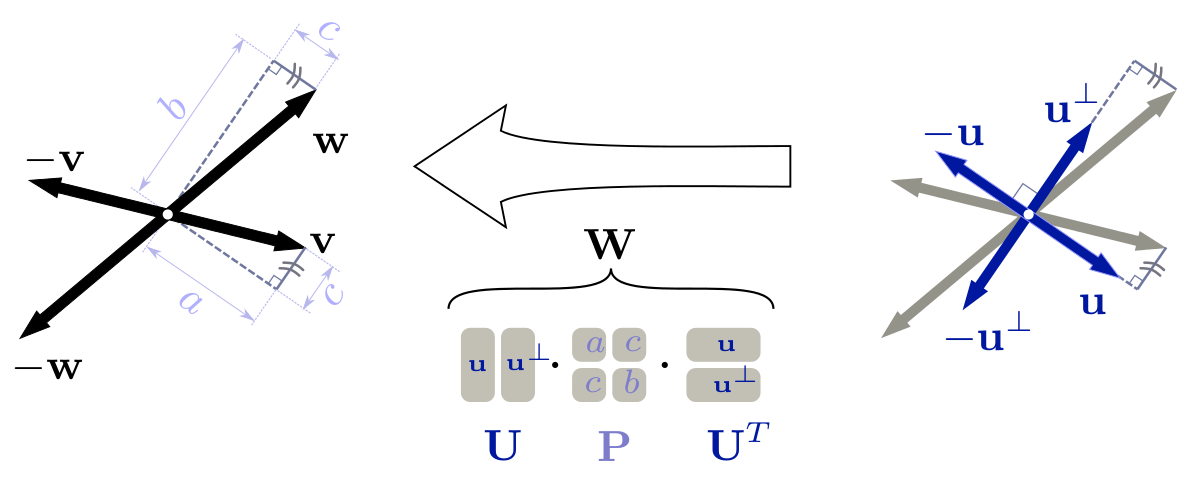
\includegraphics[width=.7\textwidth]{frame_field.png}
    \caption{Frame field示意图,图来自\cite{isotopic-appro}}
    \label{fig:frame-field}
\end{figure}
在得到一个能够充分体现原网格上的各项异性信息的标架场后,参照Daniele Panozzo等人提出方法\cite{frame-field-warping},我们通过优化标架场上的一个能量,将原标架场其变为尽可能各项同性的标架场,从而使得网格形变成为一个各项同性的网格。一个正交的标架$< u, u^\bot , −u, −u^\bot >, |u| = 1$,称为cross。我们知道对于任意的一个标架$f_p = <v, w, −v, −w >$,我们都可以在切平面$T_p S$上找到一个唯一的cross $x =<u, u^\bot , −u, −u^\bot >$和同样在该切平面上的唯一的一个线性并正定(SPD)的映射W(如图\ref{fig:frame-field}),通过它们组合表示$f_p$,$f_p = Wx = <Wu, Wu^\bot, -Wu, -Wu^\bot>$。从而,在S上的一个标架场可以唯一的分解为一个cross场$\mathcal{X}$和一个SPD张量场$\mathcal{W}$。在我们离散的三角网格上,我们将标架场离散地定义到每一个三角面片上,即每一个三角面片上均有一个标架。从而在每一个三角面片t上,我们都可以计算出一个corss $x_t$和一个由$x_t$到$f_t$映射变换$W_t$。很容易发现我们在三角面片t上的一个理想的形变是$W_t^{−1}$,这样就可以使得形变后的三角面片的local size在各个方向上都相等。然而现实中很难将所有的三角面片全部变形到最理想的状态,参照Daiele Panozzo等人的方法\cite{frame-field-warping},并根据我们的需求——需要使得主曲率方向上的local size尽可能一致,做一个修改,我们通过优化如下能量来计算每个三角面片t上的形变雅克比$J_t$:
\begin{equation}
  \epsilon(p') = \sum_{t\in S} \underset{Q_t \in SO(3)}{\text{min}} A_t \lVert J_t - sQ_t \widetilde{W_t}^{-1} \rVert_F^2
\end{equation}
这里,$Q_t$是一个3D空间中的旋转矩阵,其满足$Q_t^{-1} = Q_t$, $|Q_t| = 1$,$\widetilde{W}_t$是矩阵$W_t$的一个$3 \times 3$版本,而s则是我们为了增大解空间而加的一个放缩的自由变量——因为我们允许标架场两个方向(主曲率方向)上的相同比例的放缩,我们只期望其比例接近于1:1。在优化得到每个三角面片t上的形变雅克比$J_t$之后,我们就可以用它来计算形变之后的网格的每个顶点的新的坐标,从而我们就得到了一个各项同性的网格$M_d$(如图XXX所示)。

\subsection{改进的三角化方法}
通过上述方法,我们将一个原网格M做了一个形变,生成了一个接近各项同性的网格$M_d$。然而,这并不足以得到一个各项异性的3D三角化方法,因为我们真正想要做形变的是整一个误差空间$\Omega$,而不是原网格M。然而,对于已知M和$M_d$,去计算$\Omega$形变之后的$\Omega_d$,使得在空间$\Omega_d$上通过上述一系列简化操作后,得到的满足误差约束条件$\forall s_d \in S_d, \varepsilon(s_d)<1$的简化的网格$MS_d$,对应到原误差空间$\Omega$上得到的网格MS也仍然能够满足误差约束条件,这是一件非常具有挑战的事情。要得到形变之后的误差空间$\Omega_d$,也即需要知道形变之后的网格$M_d$上任意一处的新的误差范围。在这里我们对两个3D上的两个简单的网格椭球和圆柱做一个分析(如图XXX所示),对于三个半轴对应于x,y,z的且比例分别为1:1:4椭球,假设我们的算法非常完美,在z轴上压缩成为原来的1/4,从而得到了一个球。那么显然,对于原误差空间$\Omega$,我们也只需要将其在z轴上压缩成为原来的1/4。而对于圆柱,也假设我们的形变算法也非常完美,只是将其沿着对称轴的方向做了一个压缩,我们也只需要对其误差空间在沿着轴的方向做一个压缩。从中我们可以推测:网格$M_d$上任意一点处的误差厚度和原网格M在形变时,在该点处的曲率变化和法向上的放缩有关。而这件事情的挑战也在就在于去寻找这样一个关系,使得在形变空间$\Omega_d$上的误差约束条件和原空间$\Omega$上的误差约束条件一致。由于寻找该关系的难度很大,在这里我们使用一个更简单的替代方法,即我们根据$M \to M_d$,生成一个不那么准确地$\Omega_d'$ (按照网格整体的放缩对误差厚度做一个缩放,然后在$M_d$上以该误差厚度构建该误差空间$\Omega_d'$),得到与原空间内外壳采样点一一对应的采样点集合$S_d′$,我们在$\Omega_d'$上做3D Delaunay三角化得到$\tau′$,对应原空间中得到$\tau$,在原空间中去判断$\tau$是否满足误差约束条件。通过这种方式,我们就避免了去寻找这样一个复杂的关系,而且在得到具有各项异性的细化结果的同时,保证满足误差约束条件。

\subsection{其他细节的修改}
当用带有各项异性的三角化方法替换原3D Delaunay三角化,并解决了除了误差约束条件的判断问题之后,我们还需要对采样点的选择策略,细化过程中对于无法满足法向约束条件的四面体的处理方法做一个修改。在细化算法中,通过贪心地选取误差最大的顶点加入$\tau$中,以期快速地使得误差约束条件得到满足。不难发现,一个采样顶点的加入,会使得其周围的采样顶点的误差迅速下降,而对离其较远的区域则无影响。因此,我们认为原算法的一个假设是最大误差采样点的周围会有较多的大误差采样点。而在我们现在的算法中,由于我们使用的带有各项异性的三角化方法是在$\Omega_d$的空间中做3D Delaunay三角化,而我们在$\Omega$和$\Omega_d$上的误差函数并不完全一致(上面我们提到想要找到一个与原误差空间$\Omega$的误差函数一致的形变误差空间$\Omega_d$非常困难),因此,我们这里有两种误差:原空间上的误差和形变空间上的误差。在我们的算法中我们同时维护这两个误差,以形变空间中的误差做为优先级排序的参照,并以原空间的误差是否超过误差边界作为采样点是否需要加入四面体网格τ的判断条件。也即每次从在原空间中超过误差边界的采样点中,选取在形变空间中误差最大的采样点加入到$\tau$中。实验证明,这种策略与选取在原空间中误差最大的采样点的策略相比能够得到更好的细化结果(顶点数量更少)。另外,对于不满足法向约束条件的四面体,由于现在的三角化方法,以原来的方法——在原空间中选取离其球心最近的采样点可能无法破坏该四面体。因此,我们选取在形变空间中离该四面体球心最近的采样点加入到$\tau$中。在得到一个考虑到原网格上各项异性信息的细化结果之后,剩下的简化处理我们与原算法一致,这里不再赘述。

\section{本章小结}
在本章,我们通过对原算法的分析,发现其第一步细化并没有考虑原网格上的各项异性信息,而用了3D Delaunay三角化来构建四面体网格$\tau$。这样虽然能够获得一个质量较好地四面体网格$\tau$,但与此同时,也意味着需要通过后序的简化操作去生恢复这样的各项异性信息,而且后序的简化操作也不一定能够很好地恢复(可能会由于边的Kernel Region小,空间采样点的稀疏等原因导致有些边无法合并)。因此,我们希望能够在细化阶段将原网格上的各项异性信息利用起来,得到一个更优的细化结果,从而减少后序简化操作的负担,并优化简化结果。然后我们介绍了我们的具体做法:我们首先通过参照江腾飞等人提出的通过自定义的黎曼度量来构建标架场的方法\cite{frame-field-gen},在原网格上构建了一个体现其各项异性信息的标架场,然后依据Daniele Panozzo等人提出的基于标架场的形变算法\cite{frame-field-warping},用该标架场构建并优化一个能量,从而将带有各项异性信息的原网格M形变成为一个趋于各项同性的网格$M_d$。然后根据$M \to M_d$,在$M_d$上构建一个形变后的误差空间$Ω_d'$。通过在形变的误差空间$Ω_d'$上的3D Delaunay三角化来得到在原空间考虑到原网格上各向异性信息的三角化,从而达到了我们期望,优化了细化结果。

%\chapter{算法实现的一些细节}

\section{基本的数据操作和数据结构}
在四面体网格$\tau$的数据结构以及其上的数据操作是我们整个算法中最基础也是最重要的部分。因此,我们根据我们的需求,寻找或设计一个简单高效的四面体网格数据结构。通过对我们的算法整个过程的分析,我们将$\tau$上的数据操作分为查询和修改两类。在$\tau$上的基本查询有:遍历$\tau$上的所有顶点、所有边和所有四面体;查询一个顶点一环邻域的四面体,查询一个四面体上所有的顶点。修改操作有:添加或删除顶点;添加或删除四面体。最简单的情况下,我们可以直接用两个矩阵(一个$n \times 3$的矩阵用来存储顶点坐标,和一个$n \times 4$的矩阵用来存储四面体所包含的顶点索引)来表示一个四面体网格的数据。但是在我们的整个算法的过程中需要不断地查询脱皮信息,并改变$\tau$的拓扑结构(消边操作),这种简单的数据结构不利于我们消边操作的高效实现。受到三角网格half-edge思想的启发,针对于多面体网格的高效查询,Michael Kremer等人设计了一种half-face多面体网格结构——OpenVolumeMesh\cite{open-volume-mesh}。在half-face多面体网格结构中,包含四层基础的数据结构:vertex、half-edge、half-face和cell(多面体单元)。同时,half-face多面体的数据结构中包含两类关系信息:由上到下的关系信息和由下到上的关系信息(如图\ref{fig:half-face-top-down})。由上到下的关系信息是指对于除顶点外任意一层的元素,都包含一个用来构成它的下一层元素的一个有序列表(cell包含一个half-face的列表,half-face 包含一个half-edge的列表,half-edge包含一个vertex的列表)。由下到上的关系信息是指对于除多面体外的任意一层的元素,都包含一个需要用它来构成的更上一层的元素的有序列表(如图\ref{fig:half-face-down-top},vertex包含half-edge的一个列表,half-edge包含一个half-face的列表,half-face包含cell的列表)。另外在half-face多面网格的数据结构中,对于half-edge和half-face的每个元素中还保存了与其对立的那个half-edge和half-face。\par
\begin{figure}[htbp]
    \centering
    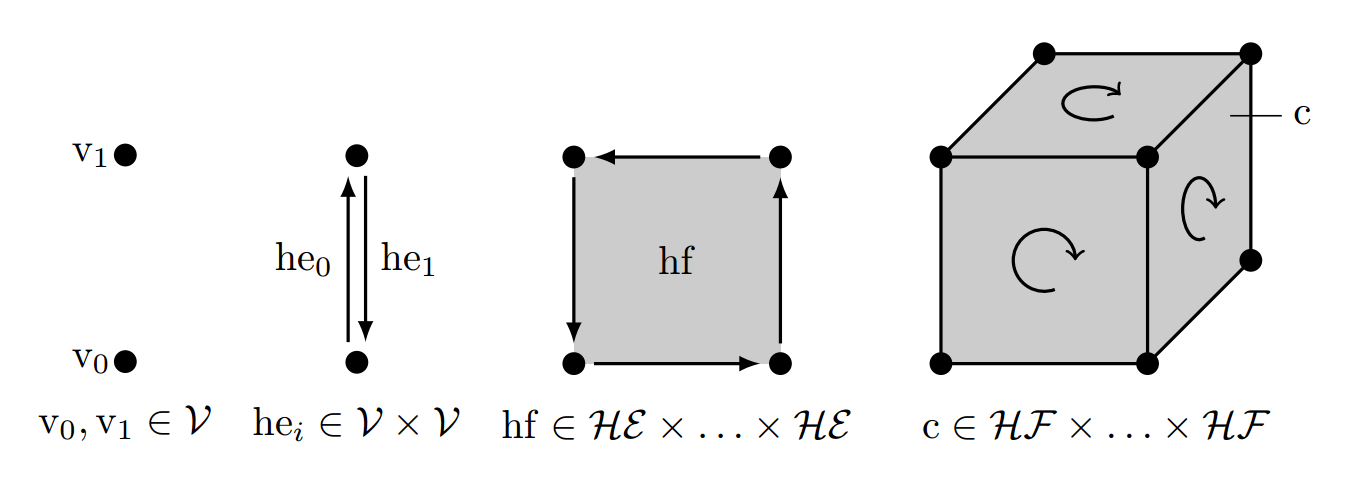
\includegraphics[width=.7\textwidth]{half-face_top_down.png}
    \caption[half-face从上到下的关系]{从上到下的关系信息示意图,对于除顶点外任意一层的元素,都包含一个用来构成它的下一层元素的一个有序列表,这些下层元素的排列顺序,决定了这个上层元素的朝向。图来自\cite{open-volume-mesh}}
    \label{fig:half-face-top-down}
\end{figure}

\begin{figure}[htbp]
    \centering
    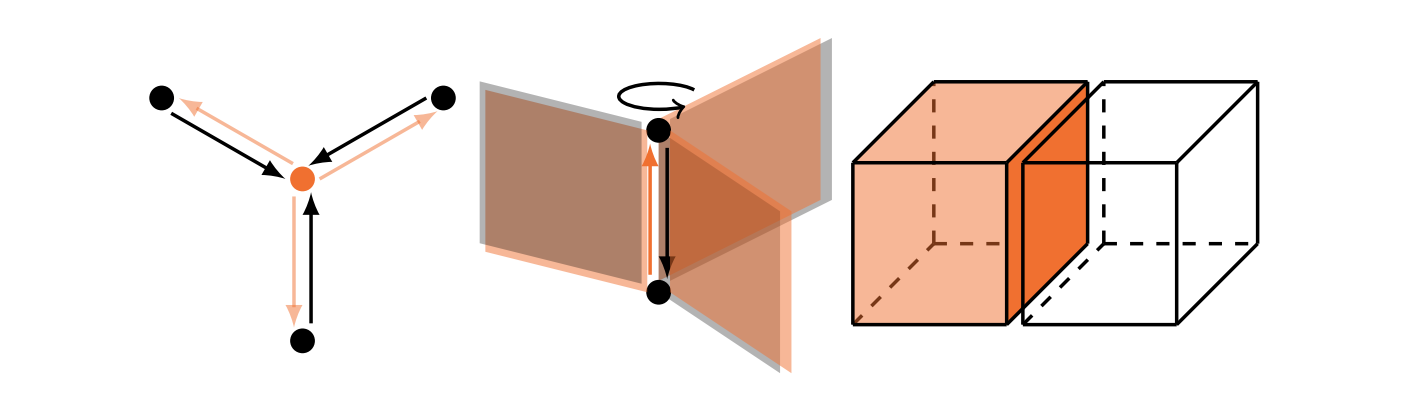
\includegraphics[width=.7\textwidth]{half-face_down_top.png}
    \caption[half-face从下到上的关系]{从下到上的关系信息示意图,对于除多面体外的任意一层的元素,都包含一个需要用它来构成的更上一层的元素的有序列表。图来自\cite{open-volume-mesh}}
    \label{fig:half-face-down-top}
\end{figure}
从上面half-face多面体网格的数据结构的描述中,我们可以看到,邻接信息的存储非常到位,对于任意一层的元素通过很少的查询,就能找到与其相邻的任意一层的元素列表,也就是说在half-face这个数据结构上信息的查询操作非常高效(比如查询一个顶点的邻接点,查询一个面的邻接多面体等等)。然而对于消边操作,由于需要维护很多的邻接关系,不仅复杂而且非常低效。\par
幸运的是,CGAL不仅给我们提供了鲁棒可靠的3D Delaunay三角化算法,而且给我们提供了一种很好的四面体网格数据结构Triangulation\_3d,其能够非常好地满足我们的需求——简单高效。在 CGAL的四面体数据结构中,包含两种最基本的数据:顶点和四面体,而边和面则通过四面体和顶点的组合来表示。对于每一个四面体,存储了该四面体的四个顶点的handle和分别与其四个面相邻接的四个四面体的handle;对于每一个顶点,存储了包含该顶点的某一个四面体的handle。通过这个简单的拓扑关系,我们就能够较为高效地查询出该四面体网格上的邻接信息,而且在做消边时也能够较为高效地维护该数据结构。

\section{密度为$\sigma$的均匀采样}
对于三角形上密度为$\sigma$的均匀采样,一种简单的均匀采样方法是为三角形做一个从全局到局部的坐标变换,使得一条边在x或y轴上,然后在其包围矩形上均匀采样,并选取属于这个三角形内的采样点(如图\ref{fig:direct-sampling-0})。但是这种方法并不鲁棒,对于有些三角形,该方法无法保证密度为$\sigma$这个条件——即以每个采样点为圆心,以$\sigma$为半径的圆能将这个三角形全部覆盖(如图\ref{fig:direct-sampling-1})。为此,我们想出了一种更好地采样方法:我们知道对于$\triangle ABC$中的任意一个采样点s都可以表示为(如图\ref{fig:param-sampling-convert}):
\begin{equation}
  \begin{split}
    s = \lambda_0 \overrightarrow{AC}+\lambda_1 \overrightarrow{AB} + A\\
    \lambda_0 + \lambda_1 \leq 1, \quad \lambda_0 \geq 0, \quad \lambda_1 \geq 0
  \end{split}
\end{equation}
因此,我们可以通过对$\lambda_0$和$\lambda_1$分别做密度为$\frac{\sigma}{\parallel \overrightarrow{AC} \parallel}$和$\frac{\sigma}{\parallel \overrightarrow{AB} \parallel}$的采样,从而间接得到$(\lambda_0,\lambda_1)$的采样,从而间接计算得到$\triangle ABC$上密度为$\sigma$的均匀采样。该采样算法能鲁棒地得到密度为$\sigma$的均匀采样(如图\ref{fig:param-sampling-0})。也可以采用相同的思想在四面体内做密度为$\sigma$的均匀采样,这里不再赘述。然而这种算法也还不够完美,采样点在三角形的边界处明显过密(如图\ref{fig:param-sampling-1})。为此,在这里使用一种基于网格细分的采样方法——对于给定的采样密度$\sigma$,我们不断遍历输入网格的每一条边,若其边长大于$\delta(\sigma)$,则我们对这条边做一个平均细分,直到所有的边的边长均小于$\delta(\sigma)$。最后我们将细分之后的三角网格上的顶点作为采样点。当$\delta(\sigma)=2\sigma/\sqrt{3}$即每一个三角形的每条边长都小于$2\sigma/\sqrt{3}$时,每一个三角形的外接圆半径小于$\sigma$,从而任一一个三角形的三个顶点上半径为$\sigma$的圆能将该三角形覆盖,从而满足采样密度要求。证明如下:设任一三角形上的最大边e的长为$x$,最大边对应的外接圆圆心角为$\alpha = 2\theta$(如图\ref{fig:max-len-calc}),则我们有
\begin{equation}
  \frac{x}{2r} = \sin\theta, \theta \in [\pi/3, \pi/2] \qquad
  \Rightarrow \qquad r =\frac{x}{2} * \frac{1}{\sin \theta} \leq \frac{x}{2} * \sqrt{3}
\end{equation}

\begin{figure}[htbp]
  \centering
  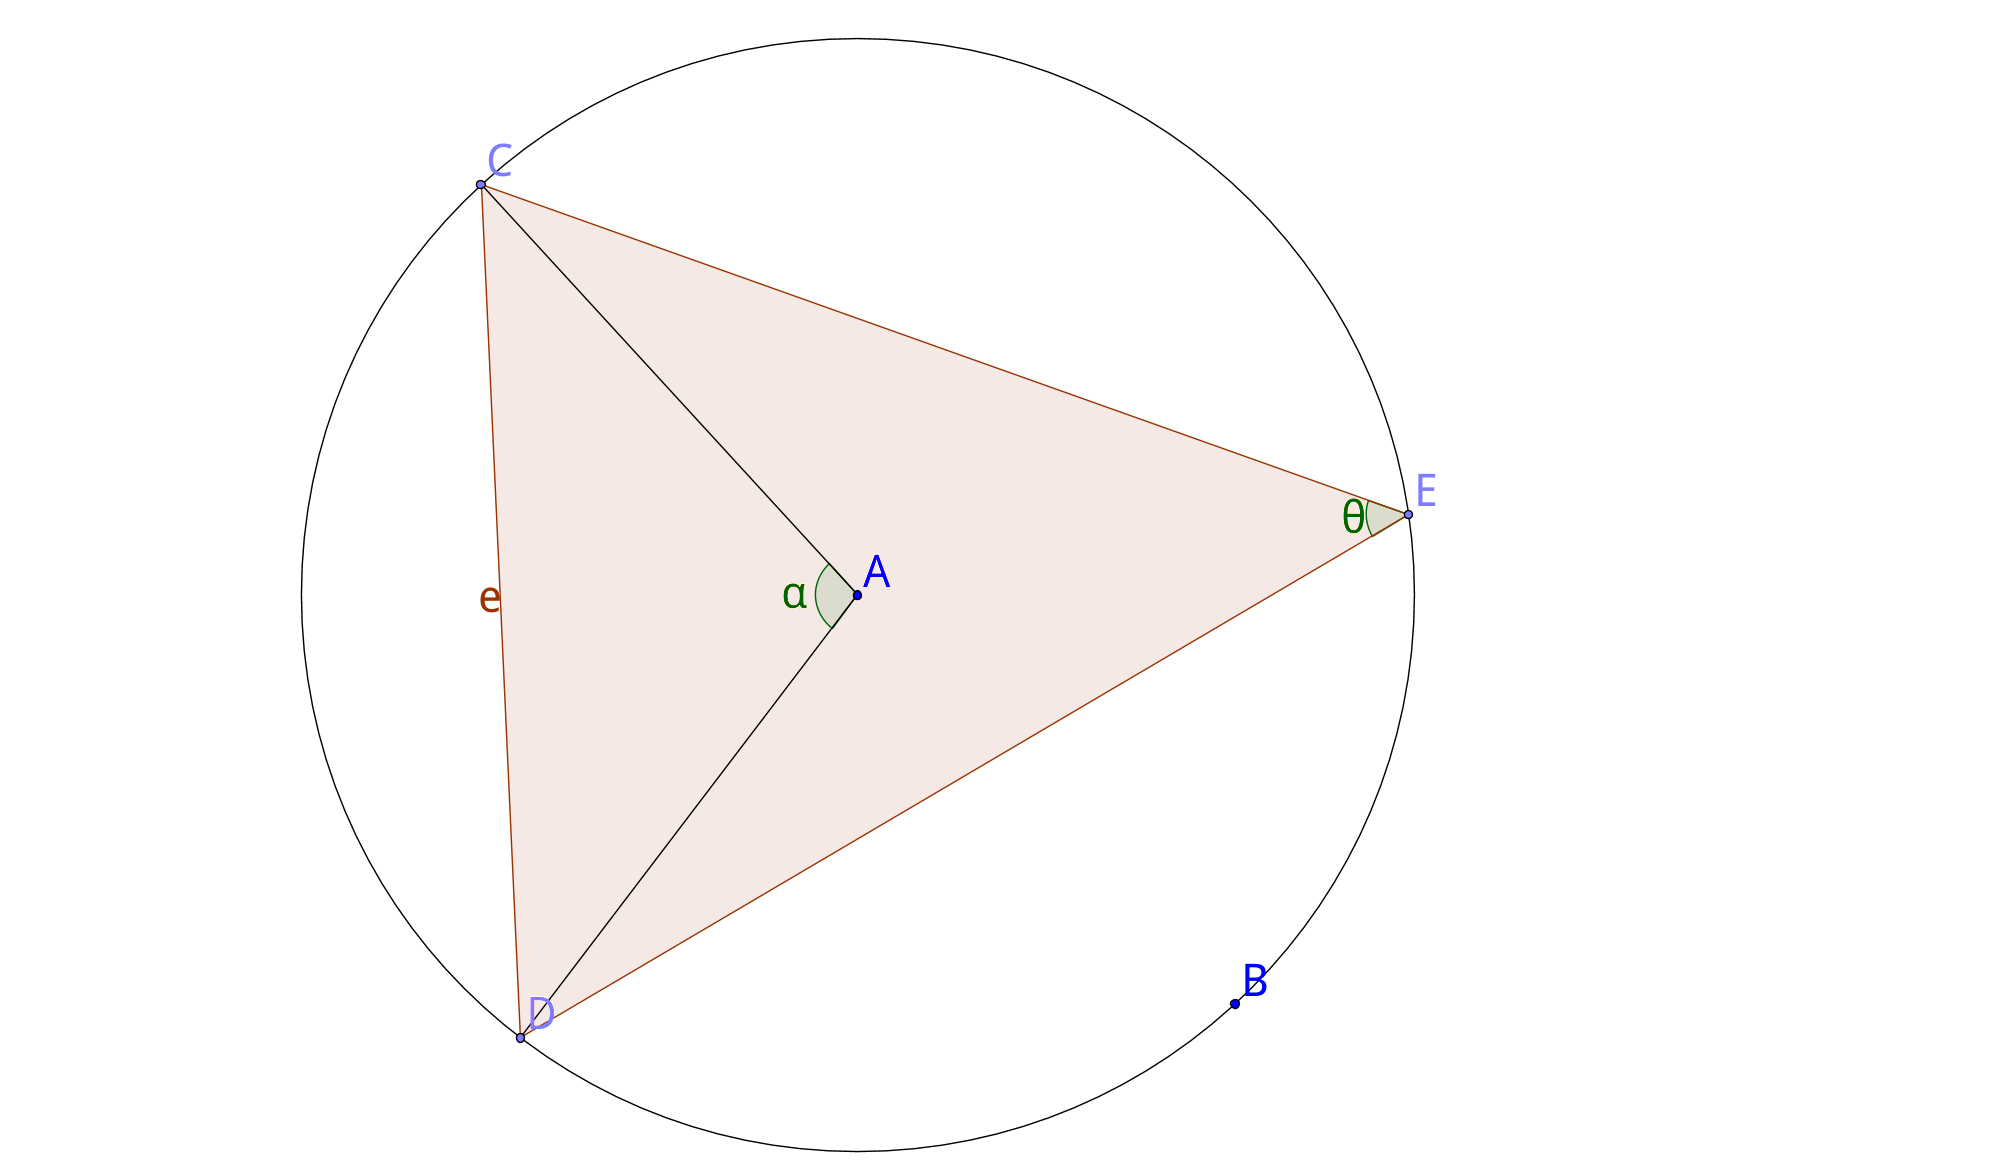
\includegraphics[width=0.8\textwidth]{max_len_calc.png}
  \caption[均匀采样细分阈值]{均匀采样时,是否需要继续细分阈值的计算示意图。}
  \label{fig:max-len-calc}
\end{figure}

\begin{figure}[htbp]
  \centering
  \begin{subfigure}[b]{0.4\textwidth}
    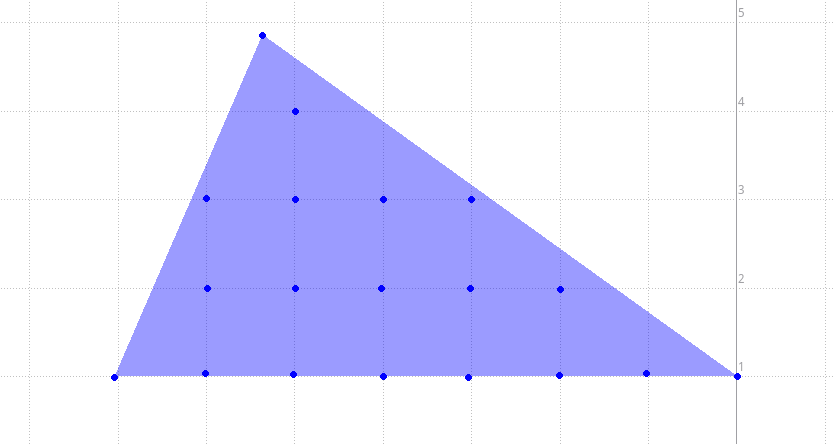
\includegraphics[width=\textwidth]{sampling_tris_basic.png}
    \caption{最直接的均匀采样方法,通过均匀撒点,然后选取在这个三角形内部的顶点作为采样结果。}
    \label{fig:direct-sampling-0}
  \end{subfigure}
  \begin{subfigure}[b]{0.8\textwidth}
      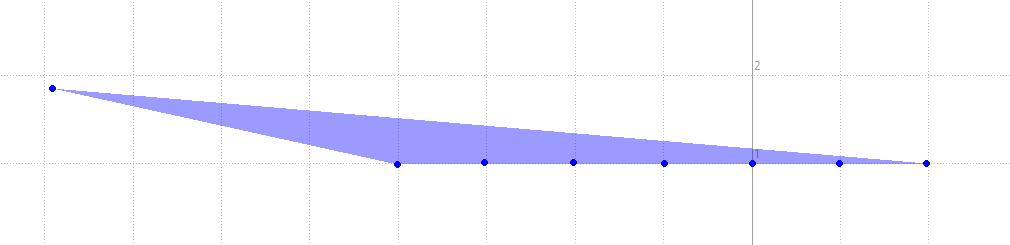
\includegraphics[width=\textwidth]{sampling_tris_fail.png}
      \caption{最直接的均匀采样方法无法保证以每一个采样点为圆心$\sigma$为半径的圆能够将整个三角形覆盖。该三角形左上方区域缺少采样点。}
    \label{fig:direct-sampling-1}
  \end{subfigure}
  \caption[最直接的采样及其问题]{最直接的均匀采样的示意图}
  \label{fig:direct-sampling}
\end{figure}

\begin{figure}[htbp]
  \centering
  \begin{subfigure}[b]{0.8\textwidth}
    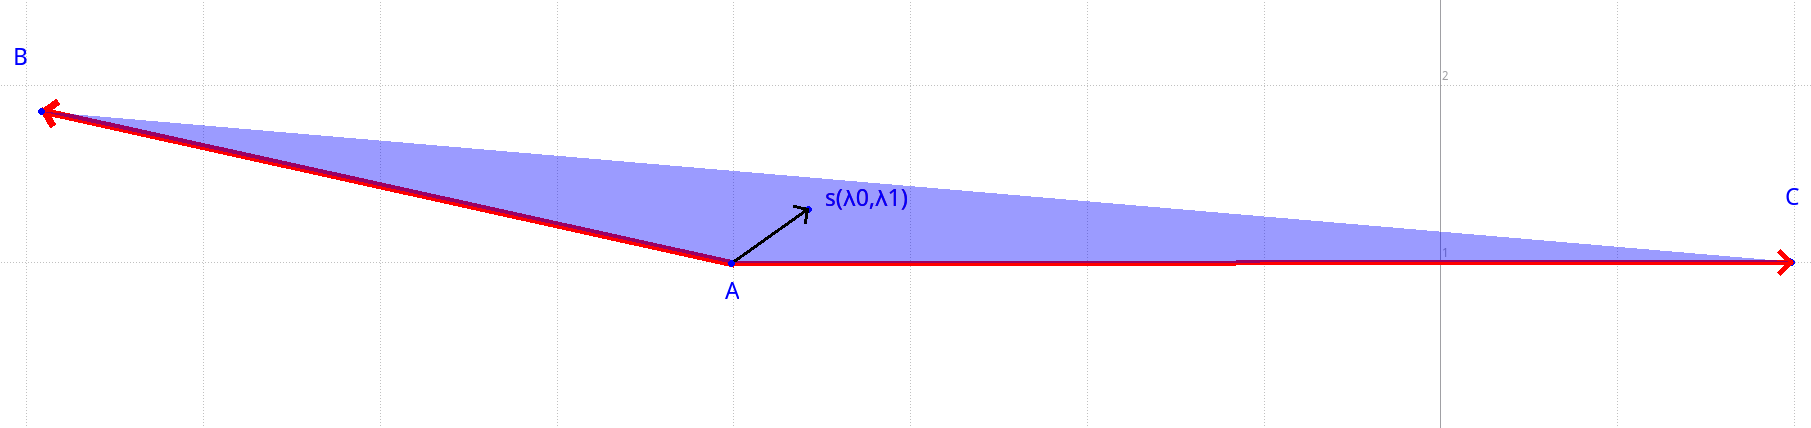
\includegraphics[width=\textwidth]{sample_tris_convert.png}
    \caption{通过对$\lambda_0$,$\lambda_1$的采样来得到该三角形的密度为$\sigma$的均匀采样。}
    \label{fig:param-sampling-convert}
  \end{subfigure}
  \begin{subfigure}[b]{0.8\textwidth}
      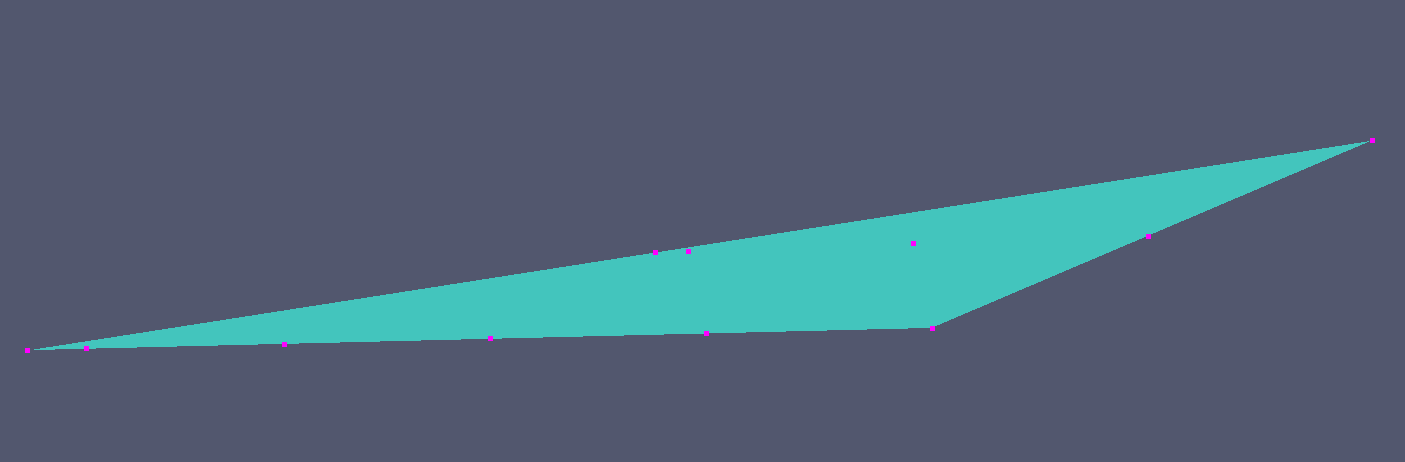
\includegraphics[width=\textwidth]{param_sampling_0.png}
      \caption{该均匀采样算法能够鲁棒地处理细长三角形,保证每一个采样点为圆心$\sigma$为半径的圆能够将整个三角形覆盖。}
      \label{fig:param-sampling-0}
  \end{subfigure}
  \begin{subfigure}[b]{0.8\textwidth}
      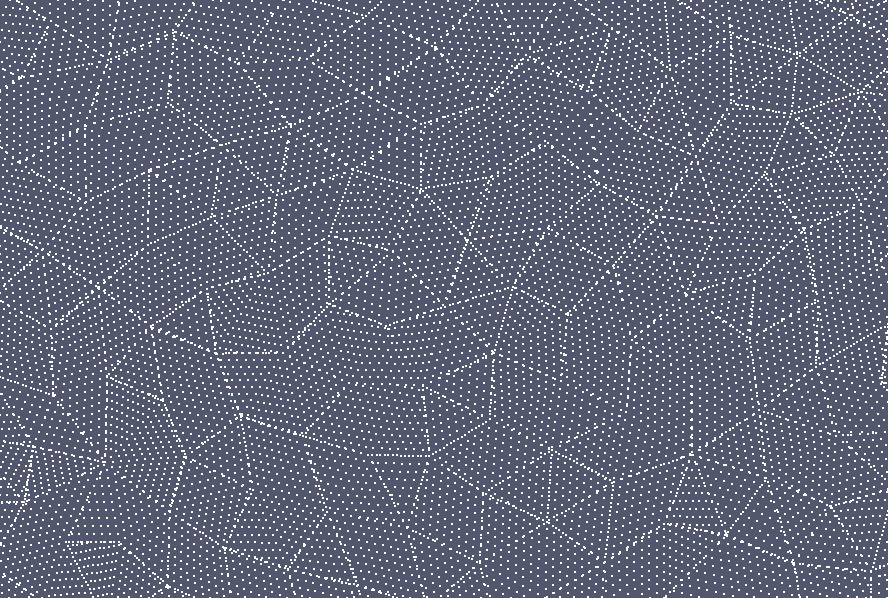
\includegraphics[width=\textwidth]{param_sampling_1.png}
      \caption{该方法的到的采样的结果,采样点在三角形的边界处明显过密。}
      \label{fig:param-sampling-1}
  \end{subfigure}
  \caption[转换参数的采样方法]{转换采样参数的均匀采样方法}
  \label{fig:param-sampling}
\end{figure}

\section{Link Condition 和 Kernel Region 的检测}
对于是否满足Link Condition,我们通过查询包含顶点A的所有四面体中,不包含顶点A的边,得到边的集合e(A),同理得到e(B),再通过查询同时包含顶点AB的四面体中,不包含顶点A和B的边得到边的集合e(AB),从而Link Condition是否满足等价于$e(A) \cap e(B) = e(AB)$是否成立。 \par
对于AB的候选合并点是否落在其Kernel Region中,即AB的一环邻域的边界的每一个三角形内侧(如图\ref{fig:kr})。邻域边界上的三角面片,即为只包含顶点A或顶点B的四面体中,除了A和B之外的另外的三个顶点所构成的三角面片。通过查询邻接信息,我们可以得到只包含顶点A或B的两个四面体集合$tet(A),tet(B)$。我们将所有这些三角面片上的一个顶点$v_i$的及其法向$n_i$(指向内侧)保存下来,然后对于每个候选合并点$v_m$判断$(v_m − v_i) \cdot n_i > 0$,即可判断其是否落在Kernel Region中。
\begin{figure}[htbp]
    \centering
    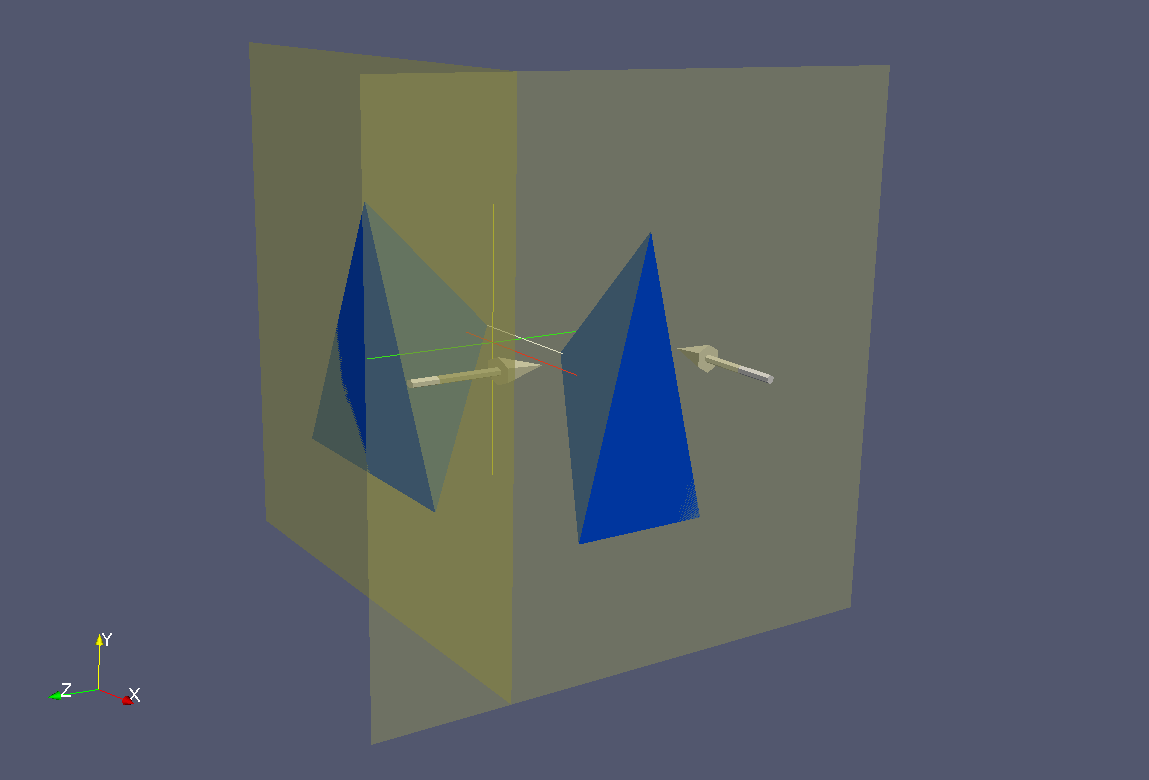
\includegraphics[width=.7\textwidth]{kr.png}
    \caption[3D Kernel Region]{对于一条边AB其Kernel Region是其一环邻域的边界上的每个三角形的内侧。图中显示了一条白色的边,以及其一环邻域中的两个四面体以及其对应的有向平面(黄色以及指向内侧的箭头),其Kernel Region是这些有向平面的内侧的交集。}
    \label{fig:kr}
\end{figure}

\section{误差判断条件的检测}
对于每一个消边后新生成的四面体$tet(v_0, v_1, v_2, v_3)$,每个采样点在这个四面体上都有唯一的重心坐标$(w_0, w_1, w_2, w_3)$。我们可以通过求解如下线性方程组来得到采样点s的重心坐标:$[v_0, v_1, v_2, v_3] \cdot [w_0, w_1, w_2, w_3]^T=s$,并根据重心坐标来判断顶点是否落在这个四面体内部——$\forall w_i>0, \sum_{i=0}^3 w_i \leq 1$,若采样点落在四面体内部,则可以可通过线性差值\eqref{eq:linear-interpolation},计算出该采样点的$\epsilon(s)$,从而判断采样点是否满足误差约束条件。

\section{消边操作}
消边操作是最基础也是重要的数据操作。在消边操作中涉及到的是操作有顶点的删除与添加、边的删除与添加、四面体的删除与添加。我们采用一种生成洞并补洞的消边方法,首先将所有包含AB的四面体从四面体网格$\tau$中移除,生成一个洞。然后再加入合并点,与该洞的边界上的面构成新的四面体,然后再更新洞的边界的四面体的邻接信息。

\chapter{结果展示}
下面我们展示我们的算法和原在一些例子上一些结果,并与原算法做一个比较,说明我们的算法的优势。我们定义误差$\delta$为该三角网格的外接球的直径的百分比。从结果中我们可以发现,我们的形变算法能够根据原网格的各项异性信息,有效地将原网格形变成为一个更趋于各项同性的网格,从而在形变之后的网格上的3D Delaunay三角化对应于原网格上则是带有其各项异性信息的三角化方法,从而优化了细化的结果,不仅减少了后序的简化操作,而且优化了简化结果。所有的实验结果均在一台CPU为Interlxxx,内存为XXX的机器上运行得到。

\section{Cylinder模型}
在一个细长的圆柱体模型(顶点数量为XX)上,我们的算法和原算法的结果对比:
\begin{figure}[htbp]
  \centering
  \begin{subfigure}[b]{0.4\textwidth}
    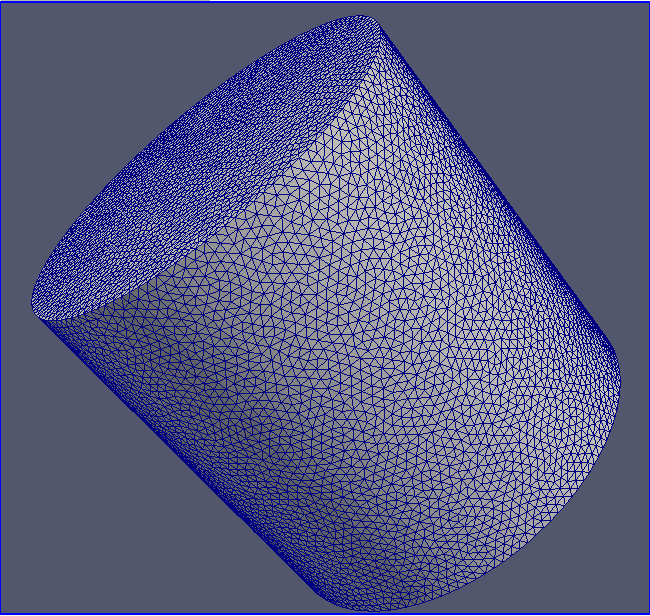
\includegraphics[width=\textwidth]{cylinder.png}
    \end{subfigure}
    \begin{subfigure}[b]{0.4\textwidth}
      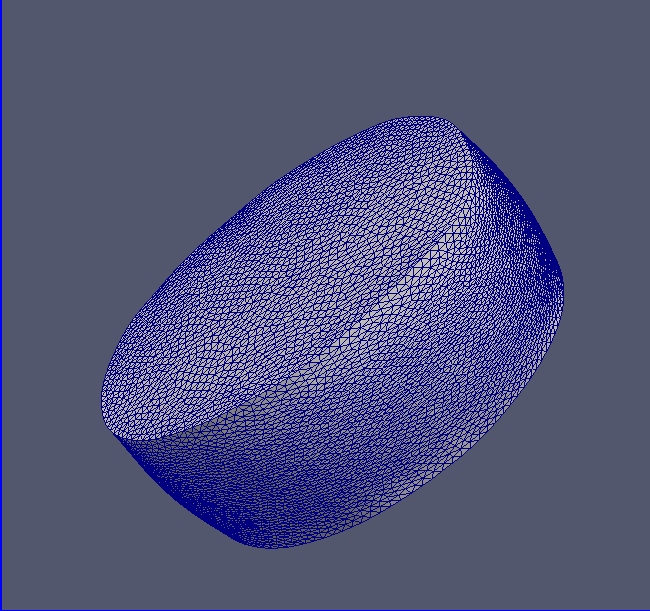
\includegraphics[width=\textwidth]{cylinder_deformed.png}
    \end{subfigure}
    \caption[Cylinder形变结果]{原网格(a)和用我们的形变算法形变之后的网格(b)}
    \label{fig:cylinder-deform}
\end{figure}


\begin{figure}[htbp]
  \centering
  \begin{subfigure}[b]{0.4\textwidth}
    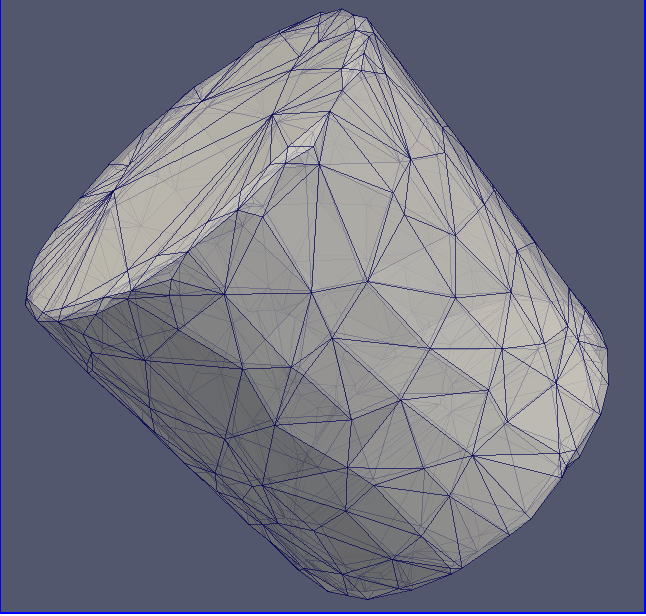
\includegraphics[width=\textwidth]{CYLINDER_0_0.02_0.02_0.04_100_refine.png}
  \end{subfigure}
  \begin{subfigure}[b]{0.4\textwidth}
    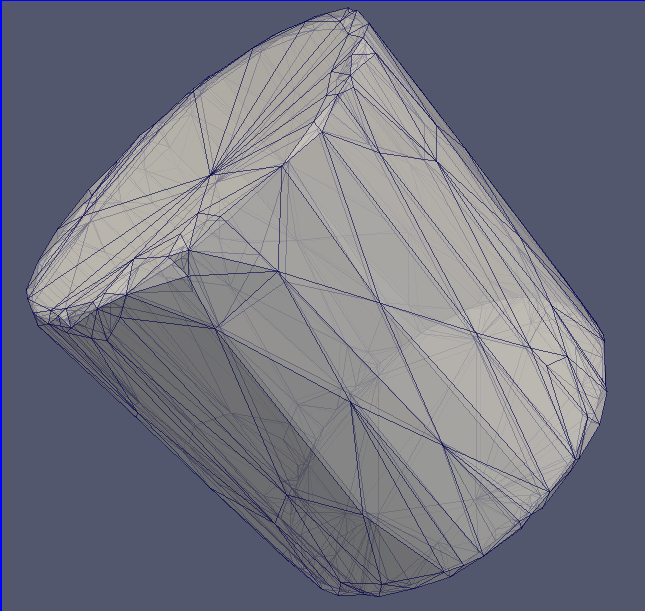
\includegraphics[width=\textwidth]{CYLINDER_1_0.02_0.02_0.04_100_refine.png}
  \end{subfigure}
  \begin{subfigure}[b]{0.4\textwidth}
    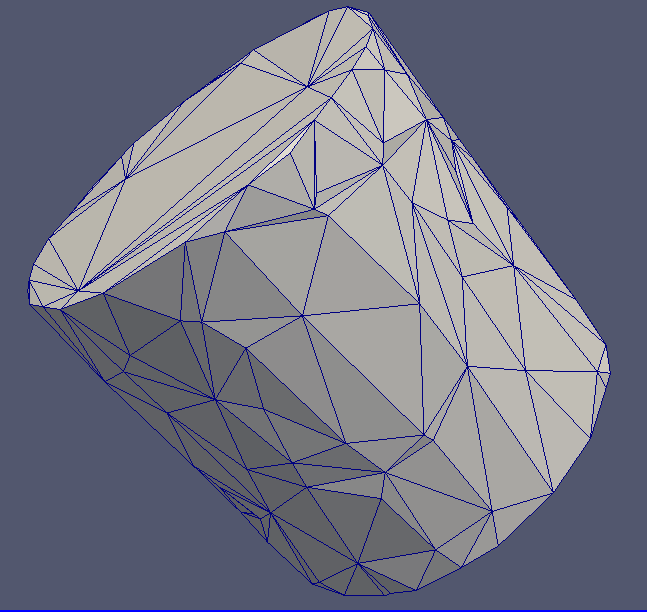
\includegraphics[width=\textwidth]{CYLINDER_0_0.02_0.02_0.04_100.png}
  \end{subfigure}
  \begin{subfigure}[b]{0.4\textwidth}
    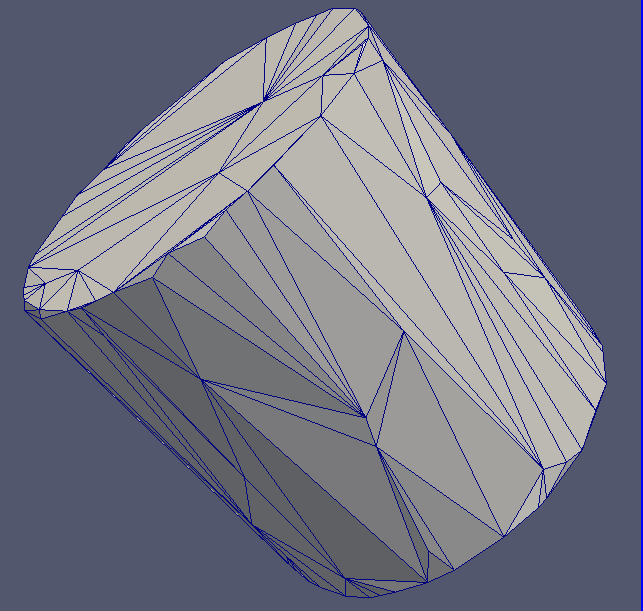
\includegraphics[width=\textwidth]{CYLINDER_1_0.02_0.02_0.04_100.png}
  \end{subfigure}
  \caption[当$\delta=0.58\%$时Cylinder结果对比]{当$\delta=0.58\%$时,原算法的细化结果(左上图)和我们的算法的细化结果(右上图),原算法的简化结果(左下图,最终顶点数量为XX)和我们的算法的简化结果(右下图,最终顶点数量为XX)}
  \label{fig:cylinder-res1}
\end{figure}

\begin{figure}[htbp]
  \centering
  \begin{subfigure}[b]{0.4\textwidth}
    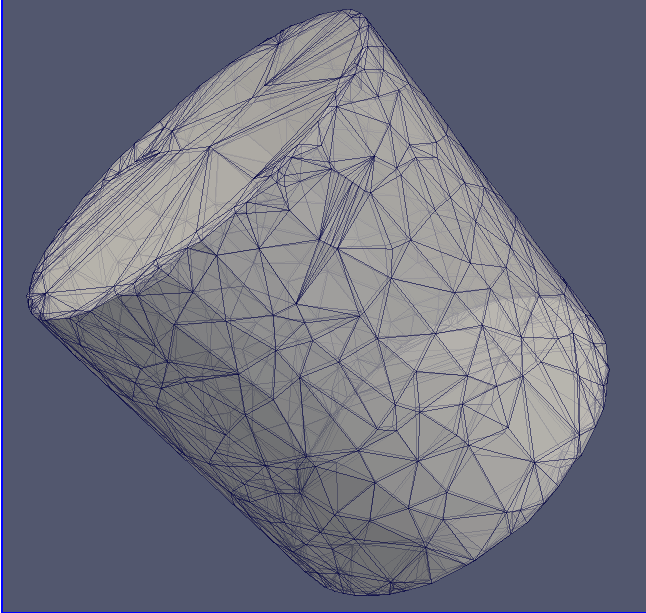
\includegraphics[width=\textwidth]{CYLINDER_0_0.01_0.005_0.02_100_refine.png}
  \end{subfigure}
  \begin{subfigure}[b]{0.4\textwidth}
    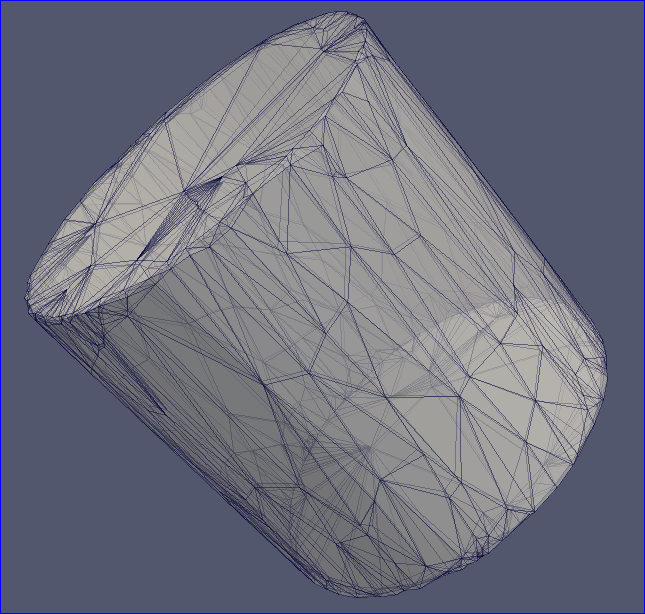
\includegraphics[width=\textwidth]{CYLINDER_1_0.01_0.005_0.02_100_refine.png}
  \end{subfigure}
  \begin{subfigure}[b]{0.4\textwidth}
    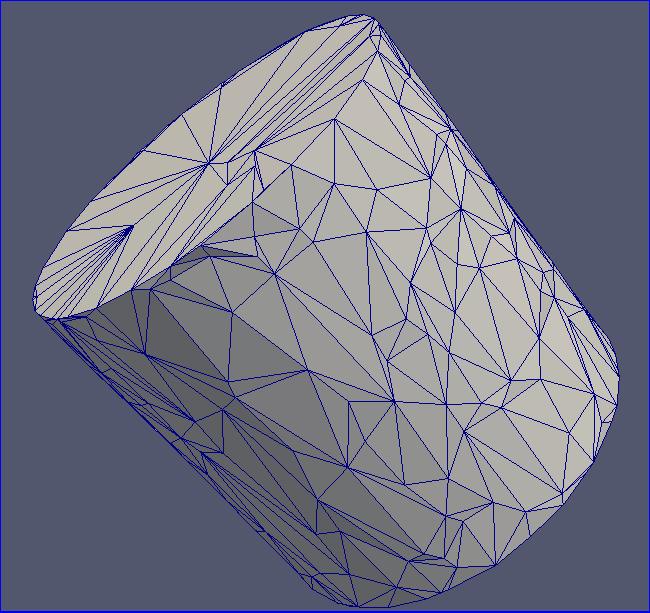
\includegraphics[width=\textwidth]{CYLINDER_0_0.01_0.005_0.02_100.png}
  \end{subfigure}
  \begin{subfigure}[b]{0.4\textwidth}
    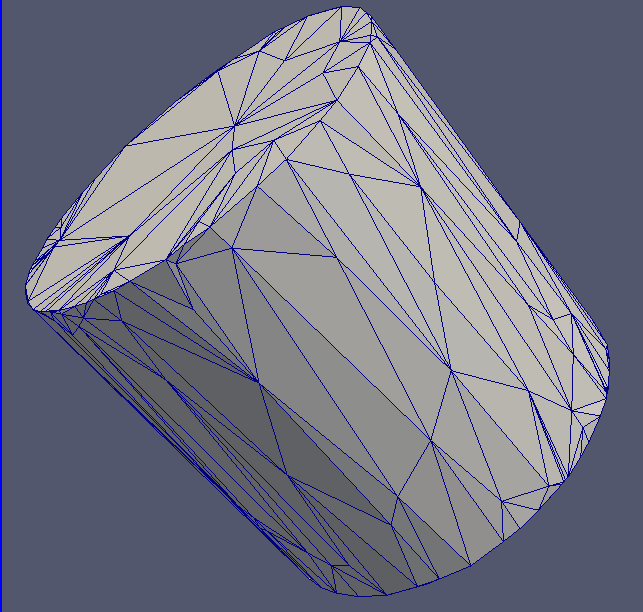
\includegraphics[width=\textwidth]{CYLINDER_1_0.01_0.005_0.02_100.png}
  \end{subfigure}
  \caption[当$\delta=0.29\%$时Cylinder结果对比]{当$\delta=0.58\%$时,原算法的细化结果(左上图)和我们的算法的细化结果(右上图),原算法的简化结果(左下图,最终顶点数量为XX)和我们的算法的简化结果(右下图,最终顶点数量为XX)}
  \label{fig:cylinder-res2}
\end{figure}

%% 原网格 - 形变之后的网格
%% \delta=? 时的对比
%% \delta=? 时的对比
%% \delta=? 时时间和顶点数量列表和原来算法的对比

\section{Cigar模型}

\section{Banana模型}

\section{Creature模型}

\section{Fertility模型}

%!TEX root = ../main.tex

\chapter{总结和展望}

\section{相关工作总结}

本模板主要内容来源于ZJU-Awesome项目,
参考软件学院论文格式要求做出调整,
并加入补充宏包,调整若干属性配置完成。
封面方面主要调整了各栏间距和对齐,
摘要依照软件学院更改了关键字的样式和页码的样式。
软件学院规定从摘要起每页必须有对应章标题的页眉,
虽然在章头处排版页眉本不雅观,
但考虑到已经有以大部分同学使用Word字处理软件遵照执行,
为保一致性,本模板暂时向软件学院的设定妥协。
由于论文格式要求并未向章头处的间距做出任何设定,
本模板保留ZJU-Awesome设定。
除此之外,本模板还做出了不少微小的改动。
详情请仔细阅读\texttt{zjuthesis.cls}和\texttt{main.tex}相关内容。

考虑到大部分软件学院的同学对\LaTeX 论文排版的陌生,
本文以尽量精炼的篇幅介绍了论文排版工作的各方面。
现在给出一个参考流程如\autoref{fig:workflow} 希望能对初次使用
\LaTeX 排版论文的同学一点提示。

\begin{figure}[htbp]
    \centering
    \includegraphics[width=.8\textwidth]{workflow.pdf}
    \caption{论文排版工作参考流程}
    \label{fig:workflow}
\end{figure}

\section{展望}

本文没有讨论各式\LaTeX 环境的使用细则,宏包的具体细节,
调试查错的技巧,也几乎没有交待任何一种具体的绘图方案。
本文希望屏幕前的你能以最少的时间代价完成论文排版工作,
养成到内容和样式完全分离的电子写作习惯,
并在对外输出知识时常思考最佳信息表达的模式。

本文草拟于2016年夏季毕业论文送审前,
希望本文能抛砖引玉。
对\LaTeX 有经验的后辈们若能继续完善甚至颠覆本模板的设定,
相信一定能对软件学院的论文排版素质起到根本的改善作用。

\section{参考文献}

\begin{description}
    \item[2] \texttt{Simplification of surface mesh using Hausdorff envelope}
    %%\item[算法宏包] \texttt{http://graphics.stanford.edu/courses/cs468-10-fall/LectureSlides/08_Simplification.pdf}
    \item[参考文献管理] \texttt{https://www.zhihu.com/question/23565739}
    \item[优雅的使用Word] \texttt{https://www.zhihu.com/question/20541531}
    \item[电子科大论文模板] \texttt{https://github.com/shifujun/UESTCthesis/wiki}
    \item[实时编译] \texttt{http://xiaoweiz.github.io/posts/2014/Aug/ST\_skim\_latexmk/}
    \item[一份不太简短的\LaTeX2e 介绍]   
    \item[各种宏包的手册] 在 TeX Live Utility 就可以查看
\end{description}
  % 总结和展望

% 结尾部分排版
\backmatter

% 引用参考文献数据库
\bibliography{references/test.bib}

% 附录部分
%\appendix
%\include{contents/appendixA}

% 作者简历
%\include{contents/self}

% 致谢
% 致谢不必感谢在下,
% 但请一定感谢清华大学薛瑞尼、
% 机械工程学院陈九历
% !TEX root = ../main.tex
\chapter{致\ZJUspace{}谢}
%% 时光荏苒,白驹过隙,提笔之际,仿佛回到了自己刚进入实验室的时候,那时的情景历历在目。在这三年的研究生生活里,我认识了很多朋友,不仅提高了自己的能力,而且端正了自己为人处世的态度,这三年的研究生生活对我的人生起到了巨大作用。

%% 我首先要感谢我的导师——黄劲教授,感谢你在这三年中的悉心教导,在学习和生活上给了我很大的帮助和指导,并对我以后的学习生活产生了很多积极的作用。黄老师勤奋刻苦的工作态度,和严谨的思考习惯给了我深刻的印象。从他那里,我学会了如何分析现象发现问题、如何解决问题。黄老师也是一个做事十分较真的人,就算是一件简单的事情,都要做到极致,让我叹为观止。

%% 同时还要感谢江腾飞、潘哲融、石泽云、张健、金耀、方贤忠、沈鑫鑫、李全、董帅等师兄(师姐)给予我的关怀和帮助,同时还要感谢陈余在学习和生活中对我的帮助,还要感谢钟俊成、陈炯、贾颜铭、王旭涛、王凯忆等师弟对我的帮助,是你们让我的研究生生活更加丰富多彩。特别感谢钟俊成和方贤忠师兄,在几何处理方向上给我的巨大帮助,帮助我并与我一起分析和研究在我遇到的难题。

%% 另外,我还要感谢我的父母,感谢你们在背后默默付出和支持。感谢我的女朋友俞春凤,给我的支持、鼓励和陪伴。是你们让我更加坚定,努力奋斗!
\vspace{2cm}
\hfill
\begin{minipage}{14em}
    \begin{flushright}
      $\quad$\\
      %% 张胜威\\
      二零一六年四月八日于求是园\\ % 学院要求的格式 - -#
      % 与封面论文提交时间一致
    \end{flushright}
\end{minipage}


\end{document}
